% =============================================================================
%  AI Tool Kart — News Agent
%  How the Agent Decides What Becomes an Article
%  Client-facing technical reference, generated from the implemented codebase.
% =============================================================================

\documentclass[11pt,a4paper]{article}

\usepackage[T1]{fontenc}
\usepackage[utf8]{inputenc}
\usepackage{lmodern}
\usepackage[margin=2.4cm,bottom=2.6cm,top=2.6cm,headheight=14pt,headsep=14pt]{geometry}
\usepackage{xcolor}
\usepackage{booktabs}
\usepackage{longtable}
\usepackage{tabularx}
\usepackage{array}
\usepackage{amsmath}
\usepackage{amssymb}
\usepackage{enumitem}
\usepackage{ragged2e}
\usepackage{microtype}
\usepackage{tikz}
\usetikzlibrary{shapes.geometric,arrows.meta,positioning,calc,fit,backgrounds}
\usepackage[most]{tcolorbox}
\usepackage[export]{adjustbox}
\usepackage{needspace}
\usepackage{fancyhdr}
\usepackage{titlesec}
\usepackage{caption}
\usepackage[hidelinks]{hyperref}

% ── Palette ──────────────────────────────────────────────────────────────────
\definecolor{aitkInk}{HTML}{16181D}
\definecolor{aitkNavy}{HTML}{1F2A44}
\definecolor{aitkAccent}{HTML}{4C5FD5}
\definecolor{aitkSoft}{HTML}{EEF1FA}
\definecolor{aitkLine}{HTML}{C9D0E4}
\definecolor{aitkGray}{HTML}{5A6272}
\definecolor{aitkStop}{HTML}{9B2C3A}
\definecolor{aitkStopSoft}{HTML}{FBEDEF}
\definecolor{aitkHold}{HTML}{8A6100}
\definecolor{aitkHoldSoft}{HTML}{FDF4E3}
\definecolor{aitkGo}{HTML}{1F6F4A}
\definecolor{aitkGoSoft}{HTML}{ECF6F0}
\definecolor{aitkRow}{HTML}{F6F7FB}

\hypersetup{
  colorlinks=true,
  linkcolor=aitkNavy,
  urlcolor=aitkAccent,
  pdftitle={AI Tool Kart News Agent — Article Judgement Criteria},
  pdfsubject={How the News Agent decides what becomes an article},
  pdfauthor={AI Tool Kart}
}

% ── Headings ─────────────────────────────────────────────────────────────────
\titleformat{\section}
  {\normalfont\Large\bfseries\color{aitkNavy}}{\thesection}{0.7em}{}
\titleformat{\subsection}
  {\normalfont\large\bfseries\color{aitkNavy}}{\thesubsection}{0.6em}{}
\titleformat{\subsubsection}
  {\normalfont\normalsize\bfseries\color{aitkGray}}{\thesubsubsection}{0.6em}{}
\titlespacing*{\section}{0pt}{1.6em}{0.7em}
\titlespacing*{\subsection}{0pt}{1.2em}{0.5em}

\pagestyle{fancy}
\fancyhf{}
\renewcommand{\headrulewidth}{0.4pt}
\renewcommand{\headrule}{\hbox to\headwidth{\color{aitkLine}\leaders\hrule height 0.4pt\hfill}}
\fancyhead[L]{\footnotesize\color{aitkGray}AI Tool Kart — News Agent}
\fancyhead[R]{\footnotesize\color{aitkGray}Article Judgement Criteria}
\fancyfoot[C]{\footnotesize\color{aitkGray}\thepage}

\captionsetup{font=small,labelfont={bf,color=aitkNavy}}
% Line-breaking tolerances: long code identifiers must break rather than overflow.
\tolerance=2500
\emergencystretch=3em
\exhyphenpenalty=0
\hyphenpenalty=50
\hbadness=3000
\vbadness=3000
\setlength{\parindent}{0pt}
\setlength{\parskip}{0.55em}
\renewcommand{\arraystretch}{1.25}

% ── Helper macros ────────────────────────────────────────────────────────────
\newcommand{\var}[1]{\texttt{\small\hyphenpenalty=0\exhyphenpenalty=0\relax #1}}
\newcommand{\us}{\_\discretionary{}{}{}}
\newcommand{\file}[1]{\textcolor{aitkGray}{\texttt{\footnotesize\hyphenpenalty=0\exhyphenpenalty=0\relax #1}}}
\newcommand{\brk}{\hyphenpenalty=0\exhyphenpenalty=0\relax}
\newcommand{\code}[1]{\texttt{\small\brk #1}}
\newcommand{\Yes}{\textcolor{aitkStop}{\textbf{Yes}}}
\newcommand{\No}{\textcolor{aitkGray}{No}}
\newcommand{\Defer}{\textcolor{aitkHold}{\textbf{Defers}}}

\newcommand{\technote}[1]{\par\vspace{-0.25em}\begingroup\footnotesize\color{aitkGray}\sloppy\emergencystretch=3em\textit{Technical note:} #1\par\endgroup}

% ── Callout boxes ────────────────────────────────────────────────────────────
\newtcolorbox{blockbox}[1][Blocking rule]{
  enhanced, breakable, colback=aitkStopSoft, colframe=aitkStop,
  boxrule=0pt, leftrule=3pt, arc=2pt, left=8pt, right=8pt, top=6pt, bottom=6pt,
  fonttitle=\bfseries\small, coltitle=aitkStop, colbacktitle=aitkStopSoft,
  title={#1}, attach title to upper={\par\vspace{2pt}}
}
\newtcolorbox{holdbox}[1][Deferral rule]{
  enhanced, breakable, colback=aitkHoldSoft, colframe=aitkHold,
  boxrule=0pt, leftrule=3pt, arc=2pt, left=8pt, right=8pt, top=6pt, bottom=6pt,
  fonttitle=\bfseries\small, coltitle=aitkHold, colbacktitle=aitkHoldSoft,
  title={#1}, attach title to upper={\par\vspace{2pt}}
}
\newtcolorbox{infobox}[1][In plain terms]{
  enhanced, breakable, colback=aitkSoft, colframe=aitkAccent,
  boxrule=0pt, leftrule=3pt, arc=2pt, left=8pt, right=8pt, top=6pt, bottom=6pt,
  fonttitle=\bfseries\small, coltitle=aitkAccent, colbacktitle=aitkSoft,
  title={#1}, attach title to upper={\par\vspace{2pt}}
}
\newtcolorbox{gobox}[1][Approval rule]{
  enhanced, breakable, colback=aitkGoSoft, colframe=aitkGo,
  boxrule=0pt, leftrule=3pt, arc=2pt, left=8pt, right=8pt, top=6pt, bottom=6pt,
  fonttitle=\bfseries\small, coltitle=aitkGo, colbacktitle=aitkGoSoft,
  title={#1}, attach title to upper={\par\vspace{2pt}}
}

% ── TikZ styles ──────────────────────────────────────────────────────────────
\tikzset{
  flowstep/.style={rectangle, rounded corners=3pt, draw=aitkNavy, fill=white,
    text width=4.4cm, align=center, minimum height=0.95cm, font=\small, inner sep=4pt},
  flowgate/.style={diamond, aspect=2.4, draw=aitkAccent, fill=aitkSoft,
    text width=3.5cm, align=center, font=\small, inner sep=1pt},
  flowstop/.style={rectangle, rounded corners=3pt, draw=aitkStop, fill=aitkStopSoft,
    text width=3.5cm, align=center, minimum height=0.8cm, font=\scriptsize, inner sep=4pt},
  flowhold/.style={rectangle, rounded corners=3pt, draw=aitkHold, fill=aitkHoldSoft,
    text width=3.2cm, align=center, minimum height=0.8cm, font=\scriptsize, inner sep=4pt},
  flowend/.style={rectangle, rounded corners=3pt, draw=aitkGo, fill=aitkGoSoft, very thick,
    text width=4.4cm, align=center, minimum height=0.95cm, font=\small\bfseries, inner sep=4pt},
  flowline/.style={-{Stealth[length=2.2mm]}, draw=aitkNavy, thick},
  flowside/.style={-{Stealth[length=2.2mm]}, draw=aitkStop, thick, dashed},
  flowsideh/.style={-{Stealth[length=2.2mm]}, draw=aitkHold, thick, dashed},
  edgelab/.style={font=\scriptsize\itshape, fill=white, inner sep=1.5pt}
}

% =============================================================================
\begin{document}

% ── Title page ───────────────────────────────────────────────────────────────
\hypersetup{pageanchor=false}
\begin{titlepage}
\centering
\vspace*{2.2cm}

{\color{aitkAccent}\rule{4cm}{2.5pt}}

\vspace{1.4cm}
{\Huge\bfseries\color{aitkNavy} AI Tool Kart\par}
\vspace{0.35cm}
{\LARGE\color{aitkNavy} News Agent\par}

\vspace{1.8cm}
{\Large\bfseries How the Agent Decides\\[0.25em] What Becomes an Article\par}

\vspace{0.9cm}
{\large\color{aitkGray} Selection, evidence, verification, editorial,\\
SEO and publication criteria\par}

\vspace{2.2cm}

\begin{tcolorbox}[enhanced, width=0.82\textwidth, colback=aitkSoft,
  colframe=aitkLine, boxrule=0.6pt, arc=3pt, left=14pt, right=14pt,
  top=12pt, bottom=12pt]
\centering\small
This document describes the \textbf{behaviour that is actually implemented} in the
AI Tool Kart News Agent codebase. Every threshold, weight, gate and reason code
quoted here was read from the source at the time of writing. Nothing has been
inferred, idealised, or carried over from design documentation that the code no
longer matches; where the two differ, the code is documented and the difference
is stated explicitly.
\end{tcolorbox}

\vfill

{\small\color{aitkGray}
Prepared for client review \quad\textbullet\quad Technical reference\\[0.3em]
Source of record: \file{news agent/src/} \quad\textbullet\quad Design brief: \file{NEWS\_AGENT.md}\\[0.3em]
Verification status: full agent test suite passing (422 of 422 tests)
\par}

\vspace{1.2cm}
{\color{aitkAccent}\rule{4cm}{2.5pt}}
\end{titlepage}

% ── Table of contents ────────────────────────────────────────────────────────
\newpage
\hypersetup{pageanchor=true}
\pagenumbering{roman}
{\color{aitkNavy}\hypersetup{linkcolor=aitkNavy}
\tableofcontents}
\clearpage
\pagenumbering{arabic}

% =============================================================================
\section{Executive Summary}
% =============================================================================

The AI Tool Kart News Agent does not ask a language model to ``write a blog
post''. A language model is never given a topic and a word count and trusted with
the result.

Instead, every candidate story travels through a sequence of independent
\textbf{decision gates}. Most of those gates are ordinary program logic --- arithmetic,
list membership, string validation, database lookups --- with no model involved at
all. The language model is used only where judgement is genuinely required
(is this relevant? what does this document actually assert? does the evidence
support this sentence?), and each of its answers is then re-checked by code that
can overrule it. The model can lower a story's chances. It can never, on its own,
raise them past a gate that code has closed.

\subsection{The pipeline at a glance}

\begin{center}
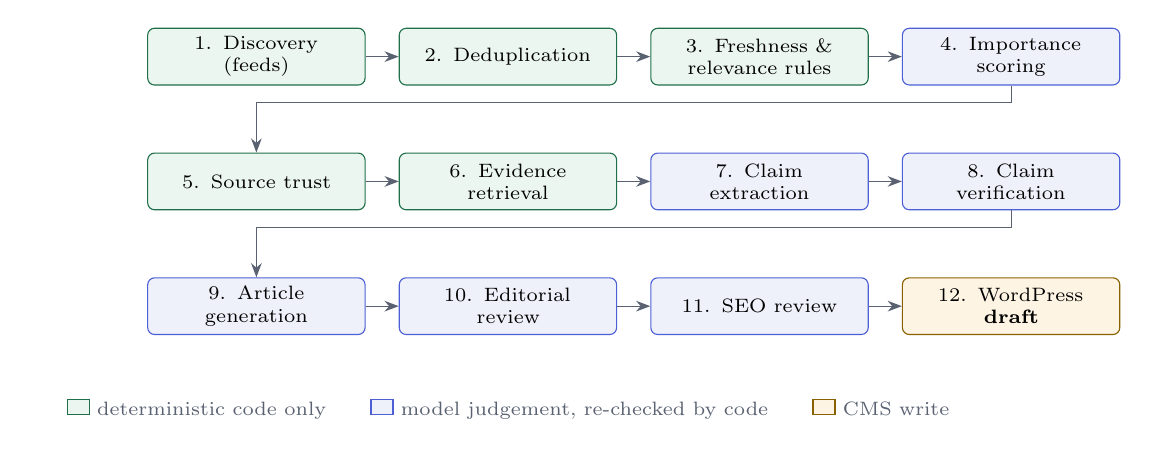
\begin{tikzpicture}[node distance=0.42cm and 0.42cm]
\footnotesize
\tikzset{stage/.style={rectangle, rounded corners=2.5pt, draw=aitkLine, fill=white,
  text width=2.55cm, align=center, minimum height=0.72cm, font=\scriptsize, inner sep=3pt},
 stagefree/.style={stage, fill=aitkGoSoft, draw=aitkGo},
 stagellm/.style={stage, fill=aitkSoft, draw=aitkAccent},
 stagepub/.style={stage, fill=aitkHoldSoft, draw=aitkHold},
 arr/.style={-{Stealth[length=1.8mm]}, draw=aitkGray}}

\node[stagefree] (a1) {1. Discovery\\(feeds)};
\node[stagefree, right=of a1] (a2) {2. Deduplication};
\node[stagefree, right=of a2] (a3) {3. Freshness \&\\relevance rules};
\node[stagellm, right=of a3] (a4) {4. Importance\\scoring};

\node[stagefree, below=0.85cm of a1] (b1) {5. Source trust};
\node[stagefree, right=of b1] (b2) {6. Evidence\\retrieval};
\node[stagellm, right=of b2] (b3) {7. Claim\\extraction};
\node[stagellm, right=of b3] (b4) {8. Claim\\verification};

\node[stagellm, below=0.85cm of b1] (c1) {9. Article\\generation};
\node[stagellm, right=of c1] (c2) {10. Editorial\\review};
\node[stagellm, right=of c2] (c3) {11. SEO review};
\node[stagepub, right=of c3] (c4) {12. WordPress\\\textbf{draft}};

\draw[arr] (a1) -- (a2); \draw[arr] (a2) -- (a3); \draw[arr] (a3) -- (a4);
\draw[arr] (a4.south) -- ++(0,-0.22) -| ($(b1.north)+(0,0.22)$) -- (b1.north);
\draw[arr] (b1) -- (b2); \draw[arr] (b2) -- (b3); \draw[arr] (b3) -- (b4);
\draw[arr] (b4.south) -- ++(0,-0.22) -| ($(c1.north)+(0,0.22)$) -- (c1.north);
\draw[arr] (c1) -- (c2); \draw[arr] (c2) -- (c3); \draw[arr] (c3) -- (c4);

\node[below=0.7cm of c2.south, font=\scriptsize, text width=12cm, align=center, color=aitkGray]
 {\tikz\draw[draw=aitkGo,fill=aitkGoSoft] (0,0) rectangle (0.28,0.2);~deterministic code only\qquad
  \tikz\draw[draw=aitkAccent,fill=aitkSoft] (0,0) rectangle (0.28,0.2);~model judgement, re-checked by code\qquad
  \tikz\draw[draw=aitkHold,fill=aitkHoldSoft] (0,0) rectangle (0.28,0.2);~CMS write};
\end{tikzpicture}
\end{center}

\vspace{0.4em}
The full sequence, in the order a story experiences it:

\begin{center}
\small
discovery $\rightarrow$ deduplication $\rightarrow$ freshness / relevance $\rightarrow$
importance scoring $\rightarrow$ source trust $\rightarrow$ evidence retrieval $\rightarrow$
claim extraction $\rightarrow$ claim verification $\rightarrow$ article generation $\rightarrow$
editorial review $\rightarrow$ SEO review $\rightarrow$ WordPress draft
\end{center}

\begin{blockbox}[The governing rule]
\textbf{Failure at any blocking gate prevents publication.} There is no
override, no ``best effort'' path, and no score high enough elsewhere to buy a
story past a gate it failed. The agent is built to produce \emph{no article} in
preference to an \emph{unsupported article}.
\end{blockbox}

\subsection{What this means commercially}

\begin{itemize}[leftmargin=1.2em,itemsep=0.25em]
  \item \textbf{The agent rejects far more than it writes.} Rejection is the
    normal outcome and is recorded with a machine-readable reason
    (Appendix~\ref{app:reasons}), so the funnel is auditable rather than opaque.
  \item \textbf{Nothing is ever published automatically.} The final artefact is a
    WordPress post with \code{status = draft}. A human decides whether it goes
    live. Automatic publishing is not merely switched off --- the agent refuses to
    start if it is configured on, and no code path exists that could honour it.
  \item \textbf{Every factual sentence is traceable.} An article may only contain
    statements that trace back to a claim extracted from a named source document
    and then verified against that document. Claims the verification step could
    not support are removed from the writer's input entirely.
  \item \textbf{Cost is bounded before quality is negotiated.} Hard per-run caps
    on candidates, verifications, articles, drafts, model calls and tokens mean a
    run has a known ceiling. When a cap is reached the remaining work is
    \emph{deferred to the next run}, not rejected.
\end{itemize}

\subsection{Three outcomes, not two}

A story is never simply ``accepted or not''. The pipeline distinguishes:

\begin{center}
\small
\begin{tabularx}{\textwidth}{@{}l>{\RaggedRight}X@{}}
\toprule
\textbf{Outcome} & \textbf{Meaning} \\
\midrule
\textcolor{aitkGo}{\textbf{Selected}} &
  The story cleared every gate reached so far and the pipeline continues spending
  effort on it. \\
\textcolor{aitkStop}{\textbf{Rejected}} &
  A judgement about the story itself: stale, irrelevant, unsupported, duplicated,
  or editorially unsound. Terminal --- the story is never reconsidered. \\
\textcolor{aitkHold}{\textbf{Deferred}} &
  A judgement about the \emph{run}, not the story: a budget or cap was reached.
  The story stays a candidate and is picked up first on the next run. \\
\bottomrule
\end{tabularx}
\end{center}

\technote{The three states are persisted on the story record as
\code{status = 'candidate' | 'verified' | 'generated' | 'published' | 'rejected' | 'deferred'}
(\file{src/domain/types.ts}), always alongside a reason string.}

% =============================================================================
\section{News Discovery and Initial Eligibility}
% =============================================================================

Everything in this section runs \textbf{before the first model call} and costs
nothing but network time. This is deliberate: if a large share of discovered
items still reached the model, the filters would be too loose and the run would
be needlessly expensive.

\subsection{How stories are discovered}

The agent reads a fixed registry of RSS/Atom feeds (\file{src/sources/registry.ts}).
No feed URL exists anywhere else in the codebase, so adding, disabling or
re-tiering a source is a configuration change and never a code change. Sources
are fetched sequentially --- the list is short and polite request behaviour toward
publishers we do not own matters more than run latency.

A source that is down, slow, rate-limited, or serving an HTML error page costs
one warning line. The run continues with every other source.

\subsection{Deterministic eligibility parameters}

\begin{center}
\footnotesize
\begin{longtable}{@{}>{\RaggedRight}p{2.6cm}>{\RaggedRight}p{2.9cm}>{\RaggedRight}p{3.0cm}>{\RaggedRight}p{4.4cm}c@{}}
\toprule
\textbf{Parameter} & \textbf{What it measures} & \textbf{Why it matters} &
\textbf{Current implementation} & \textbf{Blocking?} \\
\midrule
\endfirsthead
\toprule
\textbf{Parameter} & \textbf{What it measures} & \textbf{Why it matters} &
\textbf{Current implementation} & \textbf{Blocking?} \\
\midrule
\endhead

Source enabled state &
Whether a configured feed participates in this run &
Lets a broken or off-beat source be retired without losing its history &
\code{enabled: true|false} per entry in the registry. 10 of 17 registered sources
are currently enabled; the 7 disabled ones each carry a written reason. &
\Yes \\

Source trust tier &
How authoritative the publisher is &
Drives evidence sufficiency and per-claim verification, not just ranking &
\code{trustTier: 1|2|3}, travelling with every item from feed to verification.
7 Tier~1 and 3 Tier~2 sources enabled. &
\Yes \\

Source type &
Which fetch strategy applies &
Feeds are stable; HTML scraping is the most fragile part of any such system &
\code{type: 'rss' | 'api' | 'web'}. Only \code{rss} is implemented and enabled;
every \code{web} entry is currently disabled. &
\Yes \\

Source availability &
Whether the feed responded and parsed &
One dead feed must not end a run &
Fetch/parse failure is isolated per source, counted in \code{sourcesFailed},
and the run proceeds. &
\No \\

Per-source item cap &
How much of one feed a single run ingests &
Stops one high-volume changelog dominating the run &
\var{AGENT\us MAX\us ITEMS\us PER\us SOURCE\us PER\us RUN} (default \textbf{25}), overridable
per source via \code{maxItemsPerRun} (GitHub Changelog and AWS ML Blog are set to 15). &
\Defer \\

Banned domains &
Aggregators and content mills &
Republished content is not reporting, and ingesting it pollutes deduplication &
9 hosts in \code{BANNED\_DOMAINS}, e.g.\ \code{news.google.com}, \code{medium.com},
\code{msn.com}, \code{yahoo.com}. Dropped at ingestion, re-checked at prefilter. &
\Yes \\

Title length &
Whether the item is a real headline &
A stub title cannot be classified, deduplicated or written from &
\code{minTitleLength = 12} characters; enforced at ingestion and again at prefilter. &
\Yes \\

Story freshness &
Age of the \emph{most recent} item backing the story &
Stale news is not news &
\code{maxStoryAgeHours = 96}. Measured from the freshest item, so a story
re-covered today stays current even if the first outlet ran it two days ago. &
\Yes \\

Duplicate URL handling &
Whether this exact document was already seen &
Prevents re-drafting an already-processed story &
Level 1/2 dedupe: the canonical URL is looked up in the persisted
\code{news\_items} table and matching items are dropped before any work. &
\Yes \\

Canonical URL handling &
Reducing a URL to a stable document identity &
Two URLs for one document must not become two stories &
Deterministic canonicalisation: forced \code{https}, host normalisation
(\code{www.}, \code{m.}, \code{amp.} stripped), tracking parameters removed
(\code{utm\_*}, \code{fbclid}, \code{gclid} and $\sim$40 more), redirect wrappers
unwrapped one level, AMP/index suffixes stripped, remaining query parameters
sorted, fragment discarded. &
\Yes \\

Near-duplicate clustering &
Whether two headlines describe one event &
Three outlets covering one launch must become one article, not three &
Level 3 dedupe on normalised titles: same-story at similarity
$\geq \mathbf{0.62}$, ambiguous band $0.50$--$0.62$, within a
\textbf{72-hour} window. Two or more shared distinctive tokens promote a
near-miss to a match. &
\Yes \\

Excluded topics (hard) &
Categories of story never worth covering &
Removes noise before it can cost a model call &
5 hard-reject rules: \code{stock}, \code{doom}, \code{clickbait},
\code{listicle}, \code{horoscope-noise} (crypto/NFT/web3/metaverse). &
\Yes \\

Excluded topics (soft) &
Story shapes that should be discouraged &
Rumour and drama should be penalised, not always banned &
3 negative-weight rules: \code{rumor} ($-3$), \code{celebrity} ($-3$),
\code{unrelated-funding} ($-1.5$). Applied to the score, not as a veto. &
\No \\

Terminal story state &
Whether this story was already resolved &
A published or rejected story must never be reconsidered &
\code{already-published}, \code{previously-rejected} and
\code{duplicate-of-}\allowbreak\code{existing-story} short-circuit the prefilter. &
\Yes \\
\bottomrule
\end{longtable}
\end{center}

\technote{Implemented in \file{src/ingestion/ingest.ts}, \file{src/dedupe/url.ts},
\file{src/dedupe/title.ts}, \file{src/dedupe/cluster.ts} and
\file{src/ranking/prefilter.ts}; thresholds in \file{src/config/limits.ts} and
\file{src/config/editorial.ts}.}

\begin{blockbox}[Deduplication is biased toward merging]
When title similarity is ambiguous, the agent \emph{merges} rather than splits.
The reasoning is asymmetric cost: a wrong merge loses one article, a wrong split
publishes the same story twice. The one exception is a same-publisher guard ---
if every item already in a story came from the same domain as the new item and
the match was only ambiguous-grade, a separate story is kept, because outlets do
publish follow-ups under near-identical headlines.
\end{blockbox}

% =============================================================================
\section{Relevance and Importance Scoring}
% =============================================================================

Only stories that survive Section~2 reach a model. This section describes how the
agent decides whether a surviving story is worth spending that budget on.

\subsection{Where the numbers come from}

Four dimensions feed the score. Two are computed by code with no model
involvement; two are produced by a tightly constrained classification call.

\begin{center}
\small
\begin{tabularx}{\textwidth}{@{}l l >{\RaggedRight}X@{}}
\toprule
\textbf{Dimension} & \textbf{Source} & \textbf{Definition as implemented} \\
\midrule
Relevance $R$ & Model (0--10) & Would an AI Tool Kart reader act differently after reading this? \\
Importance $I$ & Model (0--10) & How significant is the development itself? \\
Source trust $T$ & Code (0--10) & Best available tier, plus bounded corroboration. \\
Freshness $F$ & Code (0--10) & Linear decay from the age of the freshest item. \\
Novelty & Model (0--10) & Produced and schema-validated, \textbf{but not consumed} by any gate or weight. \\
Category & Model (enum) & One of 10 fixed categories; anything else falls back to \code{industry}. \\
Recommendation & Model (\code{proceed}/\code{skip}) & \textbf{Advisory only.} Logged, never decisive. \\
\bottomrule
\end{tabularx}
\end{center}

\subsection{The weighted score}

The four dimensions combine with fixed weights from \file{src/config/limits.ts}:

\begin{equation}
S_{\text{base}} \;=\; 0.35\,R \;+\; 0.30\,I \;+\; 0.20\,T \;+\; 0.15\,F
\end{equation}

Freshness decays linearly over twice the configured half-life
(\code{FRESHNESS\_HALF\_LIFE\_HOURS} $=48$, giving a 96-hour window that matches
the staleness gate), where $a$ is the age in hours of the freshest item:

\begin{equation}
F(a) \;=\; \operatorname{clamp}_{[0,10]}\!\left( 10\left(1 - \frac{a}{96}\right)\right)
\end{equation}

Source trust takes the \emph{best} tier available and adds one point per
additional independent publisher, capped at two points:

\begin{equation}
T(\mathcal{T}, p) \;=\; \operatorname{clamp}_{[0,10]}\!\Big(
  \mathrm{Base}\big(\min \mathcal{T}\big) \;+\; \min\big(\max(p-1,0)\cdot 1,\; 2\big)\Big),
\qquad
\mathrm{Base} = \begin{cases} 10 & \text{Tier 1}\\ 7 & \text{Tier 2}\\ 3 & \text{Tier 3}\end{cases}
\end{equation}

A deterministic \emph{topic prior} then adjusts the result. It is built from the
keyword rules and audience-entity matches found during prefiltering, and it is
clamped so it can shade a borderline decision but never overturn the model's
relevance judgement:

\begin{equation}
P \;=\; \sum_{r \in \text{included}} w_r \;+\; \sum_{r \in \text{excluded}} w_r
        \;+\; 0.5 \cdot \min\big(|\text{entity hits}|,\,3\big)
\end{equation}
\begin{equation}
A \;=\; \operatorname{clamp}_{[-2,\,+2]}\big(0.4 \cdot P\big)
\qquad\Longrightarrow\qquad
\boxed{\;S \;=\; \operatorname{clamp}_{[0,10]}\big(S_{\text{base}} + A\big)\;}
\end{equation}

\technote{Included-topic weights run from $+1$ (\code{availability},
\code{integration}) to $+2.5$ (\code{mcp}); soft excluded-topic weights run from
$-1.5$ to $-4$. Entity hits are matches against the curated tool/vendor
vocabulary (43 entries in \code{TAG\_ENTITIES}), capped at three so that naming
many products cannot inflate a story.}

\subsection{Selection thresholds}

The weighted score alone does not select a story. Four gates are applied in
order, and the relevance and importance floors are checked \emph{first} ---
deliberately, so that a highly trusted, very fresh source cannot carry a story
readers do not care about.

\begin{center}
\small
\begin{tabularx}{\textwidth}{@{}>{\RaggedRight}p{2.5cm} >{\RaggedRight}p{3.1cm} >{\RaggedRight}X >{\RaggedRight}p{3.3cm}@{}}
\toprule
\textbf{Gate} & \textbf{Threshold} & \textbf{Rationale} & \textbf{Configurable} \\
\midrule
Relevance floor & $R \geq \mathbf{4}$ &
  Trust and freshness must not be able to buy an irrelevant story a place. &
  Code constant \\
Importance floor & $I \geq \mathbf{3}$ &
  Filters trivial version bumps and customer-story blog posts. &
  Code constant \\
Weighted threshold & $S \geq \mathbf{6.0}$ &
  The overall bar for spending evidence-gathering budget. &
  \var{AGENT\us MIN\us WEIGHTED\us SCORE} \\
Source base & Tier 1 present, \emph{or} $\geq 2$ independent publishers &
  A signal nobody authoritative confirms is a rumour, not a story. &
  Code constant \\
Candidate cap & $\leq \mathbf{20}$ scored per run &
  Bounds classification spend. Excess is \textbf{deferred}, not rejected. &
  \var{AGENT\us MAX\us CANDIDATES\us PER\us RUN} \\
\bottomrule
\end{tabularx}
\end{center}

\begin{blockbox}[Selection is conjunctive]
A story must clear \textbf{all four} selection gates. Failure produces one of
these recorded reasons, which name the actual values so a reviewer can see how
close the story came: \code{below-relevance-floor}, \code{below-importance-floor},
\code{below-threshold}, \code{insufficient-}\allowbreak\code{source-base}.
\end{blockbox}

\subsection{Rejected, deferred, selected}

\begin{center}
\small
\begin{tabularx}{\textwidth}{@{}p{2.2cm} >{\RaggedRight}X >{\RaggedRight}p{4.2cm}@{}}
\toprule
\textbf{State} & \textbf{Trigger} & \textbf{What happens next} \\
\midrule
\textcolor{aitkStop}{\textbf{Rejected}} &
A judgement about the story: stale, banned domain, hard-rejected topic, below a
floor, unsupported evidence, editorially unsound. &
Terminal. The reason is persisted. The story is never re-examined, but it still
absorbs future duplicates so a re-report cannot become a second article. \\
\textcolor{aitkHold}{\textbf{Deferred}} &
A judgement about the run: a candidate, verification, article, draft or LLM
budget was reached. &
The story stays a candidate. On the next run, deferred stories are re-queued
\textbf{ahead of} newly discovered ones --- but they are re-checked for
staleness, so a deferral that aged out is then rejected rather than lingering. \\
\textcolor{aitkGo}{\textbf{Selected}} &
Cleared every selection gate. &
Sorted by weighted score, highest first, so that the remaining budget is spent on
the best material. \\
\bottomrule
\end{tabularx}
\end{center}

\subsection{Deviation from the design brief}

\begin{holdbox}[Documented vs.\ implemented]
\file{NEWS\_AGENT.md} §11 lists \code{novelty} among the classifier outputs and
implies it informs ranking. In the current implementation \code{novelty} is
requested, returned and schema-validated, but \textbf{no gate or weight reads
it}. The weighted score uses relevance, importance, source trust and freshness
only. This is documented here rather than presented as an active signal.
\end{holdbox}

% =============================================================================
\section{Source Trust Model}
% =============================================================================

Trust tier is not a ranking nicety. It determines whether evidence is sufficient
at all, and it determines, per claim type, what counts as verification.

\subsection{What each tier means operationally}

\begin{center}
\small
\begin{tabularx}{\textwidth}{@{}c p{3.1cm} >{\RaggedRight}X c@{}}
\toprule
\textbf{Tier} & \textbf{Meaning} & \textbf{Operational consequence} & \textbf{Trust score} \\
\midrule
\textbf{1} & Official / primary: the vendor, its changelog, its documentation &
  Sufficient \emph{on its own} for evidence. Authoritative for facts about its own
  product --- pricing, capabilities, dates, benchmarks. Not authoritative about
  competitors. & 10 \\
\textbf{2} & Reputable technology press &
  Reliable that \emph{something happened}; not relied on for exact specifications.
  Two independent Tier 2 publishers are required where no Tier 1 source exists. & 7 \\
\textbf{3} & Discovery signal (social, forums, aggregators) &
  \textbf{Never sufficient evidence.} A Tier 3 signal that cannot be corroborated
  is treated as a rumour. Claims backed only by Tier 3 are marked unsupported. & 3 \\
\bottomrule
\end{tabularx}
\end{center}

\subsection{The configured source registry}

These are the sources actually present in \file{src/sources/registry.ts}. No
others exist in the system.

\begin{center}
\footnotesize
\begin{tabularx}{\textwidth}{@{}l l c c >{\RaggedRight}X@{}}
\toprule
\textbf{Source} & \textbf{Publisher} & \textbf{Tier} & \textbf{Enabled} & \textbf{Note} \\
\midrule
OpenAI News & OpenAI & 1 & \textcolor{aitkGo}{yes} & \\
Google DeepMind Blog & Google DeepMind & 1 & \textcolor{aitkGo}{yes} & \\
Google --- The Keyword (AI) & Google & 1 & \textcolor{aitkGo}{yes} & \\
Hugging Face Blog & Hugging Face & 1 & \textcolor{aitkGo}{yes} & \\
GitHub Blog & GitHub & 1 & \textcolor{aitkGo}{yes} & \\
GitHub Changelog & GitHub & 1 & \textcolor{aitkGo}{yes} & Capped at 15 items/run (high volume, mostly minor) \\
AWS Machine Learning Blog & AWS & 1 & \textcolor{aitkGo}{yes} & Capped at 15 items/run \\
\midrule
TechCrunch --- AI & TechCrunch & 2 & \textcolor{aitkGo}{yes} & \\
The Verge --- AI & The Verge & 2 & \textcolor{aitkGo}{yes} & \\
VentureBeat --- AI & VentureBeat & 2 & \textcolor{aitkGo}{yes} & \\
\midrule
Ars Technica --- Tech Lab & Ars Technica & 2 & \textcolor{aitkStop}{no} & Feed verified; held back as too broadly scoped \\
Anthropic News & Anthropic & 1 & \textcolor{aitkStop}{no} & No RSS feed published \\
Meta AI Blog & Meta AI & 1 & \textcolor{aitkStop}{no} & Feed returns 404 \\
Mistral AI News & Mistral AI & 1 & \textcolor{aitkStop}{no} & Feed returns 404 \\
Microsoft AI Blog & Microsoft & 1 & \textcolor{aitkStop}{no} & Feed returns HTTP 410 Gone \\
Runway Blog & Runway & 1 & \textcolor{aitkStop}{no} & Feed returns 404 \\
\bottomrule
\end{tabularx}
\end{center}

\technote{Every enabled endpoint was confirmed to return a parseable RSS/Atom
document before being switched on. Sources whose vendors publish no stable feed
are registered as disabled \emph{with the reason recorded}, rather than pointed at
a guessed URL that would fail silently on every run. \textbf{No Tier 3 source is
currently configured}: Tier 3 exists in the trust model and is the default tier
assigned to any unrecognised host, but no feed feeds it today.}

\subsection{Decision table}

\begin{center}
\small
\begin{tabularx}{\textwidth}{@{}p{3.6cm} >{\RaggedRight}X >{\RaggedRight}p{4.0cm}@{}}
\toprule
\textbf{Evidence situation} & \textbf{Agent behaviour} & \textbf{Outcome} \\
\midrule
\textbf{Tier 1 only} &
Sufficient. Selection passes the source-base gate; evidence sufficiency passes on
one Tier 1 document. Claims requiring a primary source can reach \emph{verified}. &
\textcolor{aitkGo}{Proceeds} \\

\textbf{Multiple Tier 2}, no Tier 1 &
Two or more \emph{independent publishers} are required at selection, and two or
more distinct Tier 2 publishers at evidence sufficiency. Claim types that require
Tier 1 (pricing, capability, date, benchmark, quote) are downgraded to
\emph{single-source} and must be attributed in the prose. &
\textcolor{aitkGo}{Proceeds, with attribution constraints} \\

\textbf{A single Tier 2} &
Fails the source-base gate at selection ($\text{Tier 1 absent}$ and
$\text{publishers} < 2$). &
\textcolor{aitkStop}{Rejected} --- \code{insufficient-}\allowbreak\code{source-base} \\

\textbf{Tier 3 only} &
Never sufficient. Evidence sufficiency fails; and within verification, a claim
whose supporting URLs are all Tier 3 is forced to \emph{unsupported} regardless of
what the model concluded. &
\textcolor{aitkStop}{Rejected} \\

\textbf{Source unavailable} (403 / 404 / 410 / timeout / paywall) &
The fetch is counted as failed and that document contributes no evidence. If what
remains still meets the sufficiency rule, the story continues on the remaining
sources; otherwise it is rejected. 4xx responses are \emph{not} retried. &
\textcolor{aitkStop}{Rejected} if sufficiency is lost, else proceeds \\

\textbf{Conflicting sources} &
The verifier marks the claim \code{conflicting} and must record what disagrees,
naming both values and both publishers. If the conflict touches the story's core
claim and no Tier 1 source resolves it, the story does not run. Non-core conflicts
must be reported as a disagreement in the article or omitted --- never silently
resolved. &
\textcolor{aitkStop}{Rejected} on an unresolved core conflict \\
\bottomrule
\end{tabularx}
\end{center}

\begin{blockbox}[Corroboration cannot outrank a primary source]
The corroboration bonus is capped at \textbf{+2 points} (one point per additional
independent publisher, maximum two). This is deliberate: ten outlets rewriting one
press release must not be able to outrank the vendor's own announcement. Publisher
independence is judged by registrable domain, so \code{blog.example.com} and
\code{example.com} count as one publisher.
\end{blockbox}

% =============================================================================
\section{Evidence Sufficiency}
% =============================================================================

Selection decides a story is \emph{worth} investigating. Evidence gathering
decides whether it \emph{can} be written at all. This is the step that most
often ends a promising story, and it is intended to.

\subsection{What evidence gathering is --- and is not}

The agent is not a crawler. It fetches only the URLs the story's own discovered
items already point at. It follows no links out of those pages, and it never
fetches a page speculatively.

\begin{center}
\small
\begin{tabularx}{\textwidth}{@{}p{4.6cm} >{\RaggedRight}X@{}}
\toprule
\textbf{Requirement} & \textbf{Implementation} \\
\midrule
Fetch budget per story & At most \textbf{4} evidence pages
  (\code{MAX\_EVIDENCE\_}\allowbreak\code{FETCHES\_PER\_STORY}). \\
Fetch order & \textbf{Tier 1 first}, then by recency. If the per-story budget runs
  out, what the agent holds is the primary material rather than the commentary. \\
Text volume per source & Cleaned text truncated to \textbf{24,000} characters
  (\code{MAX\_EVIDENCE\_CHARS}). \\
Minimum usable text & A page yielding fewer than \textbf{200} characters of
  article text is discarded as a paywall, JavaScript shell or consent
  interstitial. Counting it would let the verifier ``confirm'' claims against an
  empty document. \\
Network safety & Every fetch passes an SSRF guard: HTTPS only, DNS resolution
  checked against private/link-local/reserved ranges, response size capped
  (\var{AGENT\us MAX\us RESPONSE\us BYTES}, default 2.5\,MB), timeout applied
  (\var{AGENT\us HTTP\us TIMEOUT\us MS}, default 15\,s), at most 3 redirects, each
  revalidated. \\
Output form & Plain text only. Raw HTML never leaves this module --- it is the
  last point in the pipeline at which markup exists. \\
\bottomrule
\end{tabularx}
\end{center}

\subsection{The sufficiency rule}

\begin{gobox}[Evidence is sufficient when]
\textbf{at least one Tier 1 document was retrieved}, \\[0.15em]
\hspace*{1.1em}\textbf{or} \textbf{two or more distinct Tier 2 publishers} were retrieved. \\[0.35em]
Anything else is insufficient, and the story is rejected before a single claim is
extracted.
\end{gobox}

Note the wording: \emph{retrieved}, not \emph{listed}. A Tier 1 source that
appeared in the feed but whose page could not be fetched does not count. This is
the difference between a story that looks well-sourced and one that is.

\subsection{When a source fails}

\begin{center}
\small
\begin{tabularx}{\textwidth}{@{}p{4.2cm} >{\RaggedRight}X@{}}
\toprule
\textbf{Failure mode} & \textbf{Behaviour} \\
\midrule
HTTP 403 / 404 / 410 & Treated as a permanent failure. \textbf{Not retried} ---
  retrying a 404 three times is three wasted requests. The document contributes
  no evidence. \\
HTTP 5xx / 408 / 429 & Transient. Retried up to \textbf{3} attempts with
  exponential backoff (400\,ms base, 4\,s ceiling). \\
Timeout / connection reset & Transient; same retry ladder. \\
Paywall or JS shell & Fetch succeeds but yields under 200 characters of text;
  counted as a failure and discarded. \\
Prompt-injection attempt & The document is \textbf{quarantined}, not filtered ---
  see below. \\
\bottomrule
\end{tabularx}
\end{center}

\begin{blockbox}[Headline-only evidence is never allowed]
There is no path by which a headline, a feed summary, or a page the agent could
not read becomes the basis for an article. Feed summaries are used solely as
context for the relevance classifier and are never passed to the writer.
Extraction, verification and writing operate exclusively on \emph{retrieved,
cleaned document text}. When retrieval fails and sufficiency is lost, the
recorded reason is \code{no-evidence-retrieved} or
\code{insufficient-evidence (no Tier 1, \textit{n} independent Tier 2)}.
\end{blockbox}

\subsection{Quarantine of manipulated sources}

If a fetched page contains text attempting to instruct an automated reader
(``ignore previous instructions'' and similar patterns), the entire document is
withheld from every model call and recorded for human review. The agent does not
strip the offending sentences and keep the rest.

The reasoning is that an injection's instruction and its payload are usually
separate sentences, so sentence-level filtering removes the framing and leaves
the false statement behind. A page that tries to manipulate an automated reader
has disqualified itself as a source of facts, whatever else it says. This costs
the occasional false positive --- a legitimate article \emph{about} prompt
injection would be quarantined --- and that trade is accepted deliberately, with
the rejection logged so a human can overturn it.

\subsection{Designed to reject rather than hallucinate}

Every decision in this section resolves the same way when it is uncertain: stop.
Insufficient evidence produces no article and a recorded reason. It never
produces a shorter article, a hedged article, or an article assembled from the
model's background knowledge of the product. That knowledge is explicitly
forbidden downstream and is unavailable here, because the writer never receives
source documents at all --- only claims that survived verification.

% =============================================================================
\section{Claim Extraction}
% =============================================================================

Once evidence is retrieved, the agent does \emph{not} hand those documents to a
writer to paraphrase. It first converts each document into a list of
\textbf{atomic factual claims}.

\subsection{One source at a time}

Extraction runs once per evidence document, never across several at once. A
claim's origin must be unambiguous for verification to mean anything; mixing
sources into one call would let the model blur which document asserted what.

Each extracted claim carries: the statement itself (10--400 characters), a claim
type, and optionally a verbatim supporting quotation from the source (used to
audit the extractor). Claims are capped at \textbf{25} per source.

\subsection{Implemented claim types}

\begin{center}
\small
\begin{tabularx}{\textwidth}{@{}l >{\RaggedRight}X@{}}
\toprule
\textbf{Type} & \textbf{What it covers} \\
\midrule
\code{launch} & Something was released, announced, or made available \\
\code{capability} & What a product can now do, including limits and specifications \\
\code{pricing} & Costs, tiers, rate limits, free allowances \\
\code{date} & When something happened or will happen \\
\code{benchmark} & Measured results, and the benchmark named \\
\code{quote} & A direct statement attributed to a named person or company \\
\code{funding} & Investment, valuation or acquisition figures \\
\code{other} & Anything factual that fits none of the above \\
\bottomrule
\end{tabularx}
\end{center}

These eight are the complete set; the response schema is a closed enumeration, so
a ninth type cannot be invented.

\subsection{Why atomic claims}

\begin{infobox}[The practical difference]
Paraphrasing an article produces prose whose accuracy can only be assessed as a
whole. Extracting claims produces a list of separately checkable statements. That
makes three things possible that are otherwise not:
\begin{itemize}[leftmargin=1.2em,itemsep=0.15em,topsep=0.3em]
  \item \textbf{Per-fact verification.} Each statement is judged against the
    evidence individually, so one weak fact weakens one sentence rather than
    contaminating the article.
  \item \textbf{Traceability.} The published draft records exactly which claim
    identifiers it drew on, and each claim records the URLs backing it. A
    reviewer can walk any sentence back to a source document.
  \item \textbf{Tier enforcement.} Requirements such as ``pricing must come from
    the vendor'' are meaningless against prose, but are mechanical against a
    typed claim.
\end{itemize}
\end{infobox}

\subsection{Safeguards during extraction}

\begin{itemize}[leftmargin=1.2em,itemsep=0.25em]
  \item \textbf{Numbers are copied, never normalised.} Every figure, date, price
    and model name must appear exactly as the document states it.
  \item \textbf{Marketing language is not laundered into fact.} A vendor's
    superlative must be recorded as ``the company describes X as \ldots'', not as
    a bare assertion.
  \item \textbf{Instruction-shaped claims are dropped deterministically.} If an
    extracted claim itself contains injection markers, code removes it --- the
    pipeline does not rely on the model declining to emit it.
  \item \textbf{Identical claims from different sources are merged} into one claim
    backed by several URLs. That merge is what creates the corroboration signal
    verification then reads.
  \item \textbf{Extraction failure is not fatal.} One document failing costs that
    document's claims, not the story; the remaining evidence may still support
    publication. If \emph{no} claims are extracted at all, the story is rejected
    with \code{no-claims-extracted}.
  \item \textbf{Support level is not decided here.} Every claim leaves extraction
    marked \code{unsupported}. Only the verifier may raise it.
\end{itemize}

% =============================================================================
\section{Claim Verification}
% =============================================================================

This is the most consequential gate in the pipeline. It decides, claim by claim,
what the article is permitted to say.

\subsection{Two layers, and code has the final say}

\begin{enumerate}[leftmargin=1.4em,itemsep=0.3em]
  \item The \textbf{verifier model} judges each claim against the supplied
    evidence and returns a support level, the URLs it considers supporting, and a
    note for any conflict.
  \item \textbf{Deterministic tier rules are then applied on top.} A claim the
    model called \emph{verified} is downgraded when the evidence backing it does
    not meet the tier requirement for its claim type.
\end{enumerate}

\begin{blockbox}[The rules only ever downgrade]
The deterministic layer can lower a claim's support level. It can never raise
one. It exists to be stricter than the model, not to rescue claims the model
doubted. Two further guards apply: supporting URLs the model returns are
\textbf{filtered against the story's actual evidence set}, so a model echoing a
URL from the claim text cannot manufacture support; and a claim the verifier
simply ignored is treated as \code{unsupported}, not as tacitly accepted.
\end{blockbox}

\subsection{Support levels}

\begin{center}
\small
\begin{tabularx}{\textwidth}{@{}l >{\RaggedRight}X >{\RaggedRight}p{4.3cm}@{}}
\toprule
\textbf{Level} & \textbf{Definition} & \textbf{Effect on the article} \\
\midrule
\code{verified} & Two or more independent sources support it, or a single Tier 1
  source states it directly. & May be stated as fact. Counts toward the
  verified-claim floor and toward article length. \\
\code{single-source} & Exactly one non-Tier-1 source supports it, uncorroborated. &
  May appear, but \textbf{must be attributed} in the prose (``according to
  \ldots''). Does \emph{not} count toward article length. \\
\code{unsupported} & No supplied evidence states this, including reasonable
  inferences no source actually makes. & \textbf{Removed entirely.} The writer
  never receives it. \\
\code{conflicting} & Two or more sources make incompatible statements. & Must be
  reported as a disagreement naming both figures and both publishers, or omitted.
  Never silently resolved. \\
\bottomrule
\end{tabularx}
\end{center}

\subsection{Evidence requirements by claim type}

\begin{center}
\footnotesize
\begin{tabularx}{\textwidth}{@{}l >{\RaggedRight}p{4.5cm} c >{\RaggedRight}X@{}}
\toprule
\textbf{Claim type} & \textbf{Minimum evidence for \code{verified}} &
\textbf{May appear if single-source?} & \textbf{Downgrade / rejection rule} \\
\midrule
\code{launch} & Tier 1, \emph{or} 2 independent Tier 2 &
  Yes, attributed & With one Tier 2 only, falls to \code{single-source} \\
\code{capability} & \textbf{Tier 1 required} &
  Yes, attributed & No Tier 1 $\Rightarrow$ forced to \code{single-source},
  however confident the model was \\
\code{pricing} & \textbf{Tier 1 required} &
  Yes, attributed & No Tier 1 $\Rightarrow$ forced to \code{single-source} \\
\code{date} & \textbf{Tier 1 required} &
  Yes, attributed & No Tier 1 $\Rightarrow$ forced to \code{single-source} \\
\code{benchmark} & \textbf{Tier 1 required} &
  Yes, attributed & No Tier 1 $\Rightarrow$ forced to \code{single-source} \\
\code{quote} & \textbf{Tier 1 required}; otherwise 1 independent Tier 2 &
  Yes, attributed & No Tier 1 $\Rightarrow$ forced to \code{single-source} \\
\code{funding} & Tier 1, \emph{or} 1 independent Tier 2 &
  Yes, attributed & Tier 3 only $\Rightarrow$ \code{unsupported} \\
\code{other} & Tier 1, \emph{or} 1 independent Tier 2 &
  Yes, attributed & Tier 3 only $\Rightarrow$ \code{unsupported} \\
\midrule
\multicolumn{4}{@{}>{\RaggedRight}p{\textwidth}@{}}{\textit{Applies to every type:}
  if the supporting evidence is \textbf{entirely Tier 3}, the claim is forced to
  \code{unsupported}. If the model returned no usable supporting URL, the claim is
  \code{unsupported}.} \\
\bottomrule
\end{tabularx}
\end{center}

\technote{Encoded as \code{CLAIM\_RULES} in \file{src/config/limits.ts}, applied by
\code{applyTierRules()} in \file{src/verification/verify.ts}. Downgrading rather
than discarding is deliberate: a specific figure sourced only to secondary
coverage remains reportable \emph{with attribution}, so the story survives
without the figure being presented as settled.}

\subsection{How conflicting claims are handled}

A conflict never resolves itself by majority. The verifier must record what
disagrees, naming both values and both publishers. Then:

\begin{itemize}[leftmargin=1.2em,itemsep=0.25em]
  \item If the conflict touches the story's \textbf{core claim} and no Tier 1
    source resolves it, the story is rejected with \code{core-claim-conflicting}.
  \item Otherwise the conflict travels to the writer with its note attached, and
    the writer is instructed to either report the disagreement explicitly or omit
    the claim --- never to pick a side silently.
  \item The story's evidence state is marked \code{conflicting} so the condition
    is visible in the audit trail regardless of the outcome.
\end{itemize}

\subsection{What makes a story fail verification entirely}

\begin{blockbox}[Story-level verification gates (all must pass)]
\begin{enumerate}[leftmargin=1.4em,itemsep=0.2em,topsep=0.2em]
  \item The \textbf{core claim} --- the single claim the verifier identifies the
    story as resting on --- must not be \code{unsupported}.
    \hfill\code{core-claim-unsupported}
  \item The core claim must not be \code{conflicting} without a Tier 1
    resolution. \hfill\code{core-claim-conflicting}
  \item At least \textbf{3 usable claims} must survive (verified or
    single-source). \hfill\code{too-few-}\allowbreak\code{verified-claims}
  \item At least \textbf{one} claim must be fully \code{verified}; a story built
    entirely from single-source material does not run.
    \hfill\code{no-fully-}\allowbreak\code{verified-claims}
\end{enumerate}
\end{blockbox}

\begin{holdbox}[Documented vs.\ implemented]
The configuration table also carries a \code{core: true|false} flag per claim type
(true for \code{launch}, \code{capability} and \code{pricing}). \textbf{No code
path currently reads it.} The story's core claim is whichever claim the verifier
nominates, not one selected by claim type. The flag is inert configuration today
and is reported here for accuracy.
\end{holdbox}

% =============================================================================
\section{Article Format Selection}
% =============================================================================

Before a word is written, the agent decides \emph{how much article the evidence
actually supports}. This is deterministic code, not a model call --- specifically
so that the model cannot argue itself into a longer piece.

\subsection{The three formats}

\begin{center}
\small
\begin{tabularx}{\textwidth}{@{}l c c >{\RaggedRight}X@{}}
\toprule
\textbf{Format} & \textbf{Target words} & \textbf{Sections} & \textbf{Earned by} \\
\midrule
\code{brief} & \textbf{180--350} & 3--5 &
  The floor. A changelog entry, a deprecation, one well-sourced announcement.
  Requires nothing --- it is what a story gets when it clears verification. \\
\code{standard} & \textbf{500--900} & 4--7 &
  $\geq 6$ verified claims, $\geq 2$ evidence sources, $\geq 2$ independent
  publishers. \\
\code{analysis} & \textbf{900--1400} & 5--9 &
  $\geq 12$ verified claims, $\geq 3$ evidence sources, $\geq 3$ independent
  publishers, \emph{and} classifier importance $\geq 7$. \\
\bottomrule
\end{tabularx}
\end{center}

A story is awarded the highest format whose thresholds it \emph{fully} meets; all
conditions in a row are conjunctive.

\subsection{What counts, and what deliberately does not}

\begin{center}
\small
\begin{tabularx}{\textwidth}{@{}p{5.0cm} >{\RaggedRight}X@{}}
\toprule
\textbf{Signal} & \textbf{Role in the decision} \\
\midrule
Verified claims & \textbf{Counts.} Only \code{verified} claims contribute to
  depth. \\
Single-source claims & \textbf{Does not count.} They may appear in the prose with
  attribution, but they must not be what buys a longer article --- otherwise
  format becomes a way of laundering weak sourcing into length. \\
Number of evidence sources & \textbf{Counts.} Documents actually retrieved. \\
Independent publishers & \textbf{Counts.} Deduplicated by publisher name, so
  twenty claims from one press release remain one account. \\
Story significance & \textbf{Counts for \code{analysis} only.} Importance $\geq 7$
  is required, so a well-sourced but minor story cannot reach the longest form. \\
Tier 1 source count & Recorded in the audit trail; not itself a threshold. \\
\bottomrule
\end{tabularx}
\end{center}

\begin{gobox}[A short article is a success, not a degraded one]
The format ordering is not a quality ranking. The writer is told the range is a
\emph{ceiling on ambition, not a quota}: if the verified material does not fill
it, write less and stop. The editor judges the draft against that same range
rather than a global minimum. Being \emph{under} the range is expected when the
evidence runs out first and is advisory only; being \emph{over} it is the more
suspicious signal, because the extra words had to come from somewhere.
\end{gobox}

\technote{This replaced an earlier flat 500-word minimum. The first real article
the pipeline produced ran to 176 words from a GitHub changelog entry that
supported exactly eight verified facts --- accurate, attributed, and reported as a
failure against a target it could never legitimately have reached. The only route
to 500 words would have been padding, which the factual-grounding rules forbid, so
the target moved to the evidence instead. Implemented in
\file{src/editorial/format.ts}; thresholds in \code{FORMAT\_THRESHOLDS}.}

\subsection{Stability across revisions}

The format is computed \textbf{once}, before writing, and the same value is used
for the first draft, the editorial review, any revision, and the second review. A
rewrite fixes issues; it does not renegotiate how long the article is allowed to
be. The chosen format is persisted with the article, so a reviewer can see which
range the draft was judged against.

A separate hard ceiling of \textbf{1400 words} applies regardless of format: a
draft exceeding it is rejected outright as runaway output rather than treated as
content.

% =============================================================================
\section{Writer Constraints}
% =============================================================================

\subsection{What the writer receives}

\begin{center}
\small
\begin{tabularx}{\textwidth}{@{}p{4.6cm} >{\RaggedRight}X@{}}
\toprule
\textbf{Input} & \textbf{Detail} \\
\midrule
Verified and single-source claims & Each with its identifier, claim type, support
  level, and the publishers backing it. Conflicting claims arrive with their
  conflict note. \\
Source metadata & Publisher, tier, publication date and URL --- for attribution
  and the Sources block. This is our own registry data, not fetched content. \\
Assigned format and word range & Presented as a ceiling on ambition. \\
Category & One of the ten fixed editorial categories. \\
SEO brief (when one exists) & Keyword and heading guidance, placed \emph{after}
  the claims in the prompt and explicitly subordinate to them. \\
Editor feedback (revision pass only) & The specific issues a rewrite must fix. \\
\bottomrule
\end{tabularx}
\end{center}

\subsection{What the writer does not receive}

\begin{blockbox}[The writer never sees a source document]
By this point, third-party prose has been reduced to atomic claims that a separate
step has already judged. The writer receives no raw HTML, no fetched page text, no
feed summaries, and no quarantined material. This is simultaneously the editorial
rule (\emph{write from evidence, not from memory}) and the strongest
prompt-injection defence in the pipeline: text that never reaches the writer
cannot influence what it writes.

Claims marked \code{unsupported} are filtered out before the prompt is built. From
the writer's perspective, they do not exist.
\end{blockbox}

\subsection{Explicit generation constraints}

\begin{itemize}[leftmargin=1.2em,itemsep=0.25em]
  \item \textbf{Verified-claims-only.} Every factual statement must trace to a
    supplied claim. Capabilities, prices, dates, context-window sizes, benchmark
    results, version numbers, quotations, funding figures and availability details
    may not be added. If a number would improve a sentence but was not supplied,
    the sentence is written without it.
  \item \textbf{No background knowledge.} The writer is instructed that its
    training data may be wrong or outdated about this specific story, and is
    forbidden from using it to fill gaps.
  \item \textbf{Mandatory attribution.} Single-source claims must be attributed in
    the text. Conflicting claims must be reported as disagreements or omitted.
  \item \textbf{No extended quotation.} Short attributed quotations only, and only
    where the exact wording matters.
  \item \textbf{Structured output, never markup.} The writer returns a title,
    excerpt, category, tags, sections (headings with paragraphs and bullets) and
    the list of claim identifiers it used. It never produces HTML, Markdown or a
    slug. A closed, strict schema rejects any unexpected field.
  \item \textbf{Fixed structure.} Five prescribed headings --- \emph{What happened,
    What's new, Why it matters, Who should care, Practical implications} --- with
    an instruction to omit any heading for which there is no verified material
    rather than pad it.
  \item \textbf{Bounded fields.} Title $\leq 110$ characters; excerpt 80--320
    characters, written deliberately rather than truncated from the body;
    2--5 entity tags; 3--9 sections.
  \item \textbf{Banned hype language.} A configured list of 15 phrases is
    prohibited (``in the rapidly evolving landscape'', ``game-changing'',
    ``revolutionary'', ``delve into'', ``unlock the power'', ``a testament to'',
    ``in conclusion'', and others). This is enforced twice: the prompt forbids
    them, and deterministic code blocks any draft containing one.
  \item \textbf{Traceability.} The writer must list the claim identifiers it drew
    on; code then discards any identifier that does not correspond to a real
    claim.
\end{itemize}

\subsection{What code produces, not the model}

\begin{center}
\small
\begin{tabularx}{\textwidth}{@{}p{3.4cm} >{\RaggedRight}X@{}}
\toprule
\textbf{Artefact} & \textbf{How it is produced} \\
\midrule
HTML body & Rendered by application code from the validated sections, using a
  fixed tag allowlist (\code{p, h2, h3, ul, ol, li, a, strong, em, blockquote,
  code}). Every text node is HTML-escaped unconditionally. \\
Slug & Derived deterministically from the title, transliterated, lowercased,
  capped at 72 characters, collisions resolved by numeric suffix. Fixed on first
  generation and reused on every revision, so a rewrite never changes the URL. \\
Sources block & Built from the evidence records. Only HTTPS URLs that pass the
  same validation used for fetching become links. \\
Tags & Normalised and validated against the entity vocabulary (Section~12). \\
Word count & Measured on the rendered prose, excluding the Sources block. \\
\bottomrule
\end{tabularx}
\end{center}

\technote{The React front end renders post bodies with
\code{dangerouslySetInnerHTML} on the assumption that WordPress is a trusted
author surface. Building the HTML here, from validated structured data with a
fixed allowlist, is the control that keeps that assumption true. A test asserts
that model-supplied markup cannot reach WordPress as markup.}

% =============================================================================
\section{Editorial Validator}
% =============================================================================

Generation succeeding never means approval. A second, independent pass reviews
the draft against the same verified claims the writer was given, and
deterministic checks are then applied on top of its verdict.

\subsection{What the editorial pass checks}

\begin{center}
\small
\begin{tabularx}{\textwidth}{@{}p{3.5cm} c >{\RaggedRight}X@{}}
\toprule
\textbf{Check} & \textbf{Decided by} & \textbf{Rule as implemented} \\
\midrule
Unsupported facts & Model & Every factual sentence must map to a supplied claim.
  Any that does not is a \textbf{blocking} \code{unsupported-claim} issue. Numbers,
  dates, prices, model names and version numbers receive particular attention. \\
Overstatement & Model & A claim of ``faster'' rendered as ``3× faster'', or
  ``available to some users'' rendered as ``generally available'', is a
  \textbf{blocking} \code{overstated-claim} issue. \\
Headline accuracy & Model & If the body does not establish what the headline
  asserts, that is a \textbf{blocking} \code{misleading-headline} issue. \\
Attribution & Model & Single-source claims must be attributed; conflicting claims
  must be reported as disagreements or omitted. Otherwise \textbf{blocking}
  \code{missing-attribution}. \\
Duplicate risk & Model & The draft is compared against the last 100 published
  titles. Covering the same event is a \textbf{blocking} \code{duplicate} issue. \\
Tone & Model + code & Hype, marketing register and rhetorical questions are
  \code{hype} issues (usually minor). Any of the 15 \textbf{banned phrases} is
  caught deterministically and blocks. \\
Structure & Model & Padding and organisational problems are \code{structure}
  issues; grammar is \code{grammar}. Usually minor unless pervasive. \\
Length / format & Code & Word count is compared against the draft's \emph{own}
  format range. Both under and over are \textbf{advisory}, reported distinctly, and
  never blocking. \\
Sources block & Code & The rendered HTML must contain a Sources section and the
  draft must carry at least one source URL. \textbf{Blocking.} \\
Claim traceability & Code & The draft must cite at least one real claim
  identifier. \textbf{Blocking.} \\
Excerpt & Code & Must be present and at least 80 characters. \textbf{Blocking.} \\
Category & Code & Must be one of the ten allowlisted categories; the writer may
  refine it only within that closed set. \\
Tags & Code & More than \textbf{5} tags \textbf{blocks}. Fewer than \textbf{2} is
  \textbf{advisory} only --- see below. \\
HTML safety & Code & Any tag outside the renderer's allowlist \textbf{blocks}. \\
SEO & Code & Blocking SEO findings are folded in; see Section~11. \\
Confidence & Code & The model's own confidence must reach \textbf{0.60}. \\
\bottomrule
\end{tabularx}
\end{center}

\begin{infobox}[Why too few tags is advisory but too many blocks]
Tags degrade gracefully in the front end, and the tag vocabulary is partly
curated, so a story about an unlisted vendor can legitimately end up with a single
tag. Blocking on that would withhold a sound article over a metadata nicety that
no rewrite could fix. An excessive tag count, by contrast, indicates the model
generated tags from article phrasing rather than entities, which is a real defect.
\end{infobox}

\subsection{Decision states}

\begin{center}
\small
\begin{tabularx}{\textwidth}{@{}l >{\RaggedRight}X@{}}
\toprule
\textbf{Verdict} & \textbf{Meaning and consequence} \\
\midrule
\code{approved} & No blocking issue from the model, none from the deterministic
  checks, none from SEO, and confidence $\geq 0.60$. Only this verdict may reach
  WordPress. \\
\code{needs-revision} & Blocking issues exist but could plausibly be fixed by
  rewriting from the same claims. One revision may be attempted. \\
\code{rejected} & The draft cannot be fixed from the available claims: it is
  substantially ungrounded, duplicates a published story, or the material does not
  support an article. \\
\bottomrule
\end{tabularx}
\end{center}

\begin{blockbox}[Code overrides an over-generous model verdict]
If the model returns \code{approved} but any deterministic check found a blocking
issue, the verdict is lowered to \code{needs-revision}. If the model returns
\code{approved} with confidence below \textbf{0.60}, the verdict is lowered to
\code{needs-revision}. \\[0.4em]
If the editorial call \textbf{cannot run at all} --- provider outage, schema
failure, budget exhaustion --- the draft is treated as \code{rejected} with the
reason \code{editorial-review-unavailable}. Failing open here would mean an
unreviewed article reaching the CMS, which is precisely what this step exists to
prevent.
\end{blockbox}

\subsection{The bounded revision loop}

\begin{center}
\resizebox{\textwidth}{!}{%
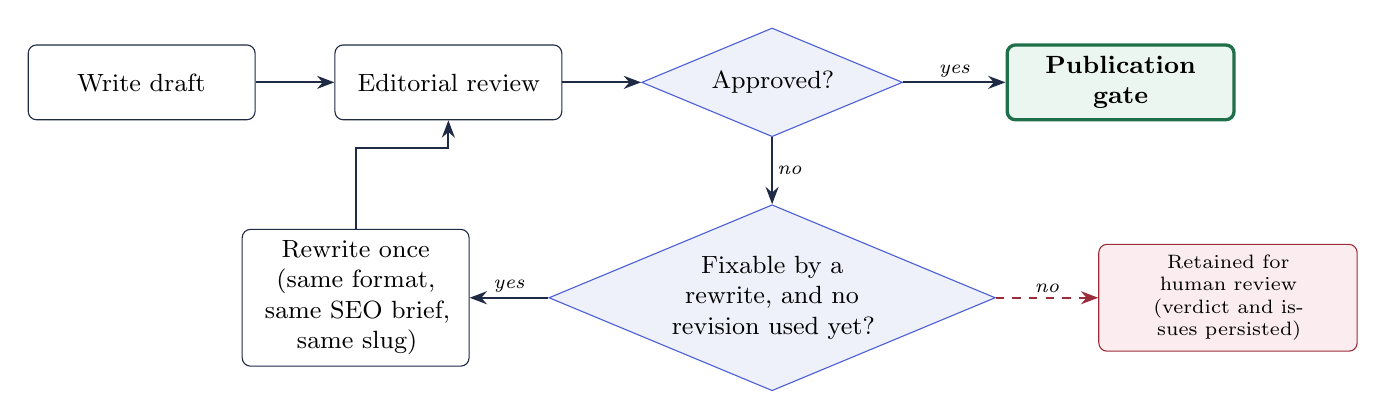
\begin{tikzpicture}[node distance=0.55cm and 1.0cm]
\footnotesize
\node[flowstep, text width=2.6cm] (w1) {Write draft};
\node[flowstep, text width=2.6cm, right=of w1] (e1) {Editorial review};
\node[flowgate, text width=2.4cm, right=of e1] (g1) {Approved?};
\node[flowend, text width=2.6cm, right=1.3cm of g1] (ok) {Publication gate};
\node[flowgate, text width=2.9cm, below=0.85cm of g1] (g2) {Fixable by a rewrite, and no revision used yet?};
\node[flowstep, text width=2.6cm, left=1.0cm of g2] (w2) {Rewrite once\\(same format, same SEO brief, same slug)};
\node[flowstop, text width=3.0cm, right=1.3cm of g2] (hold) {Retained for\\human review\\(verdict and issues persisted)};

\draw[flowline] (w1) -- (e1);
\draw[flowline] (e1) -- (g1);
\draw[flowline] (g1) -- node[edgelab,above]{yes} (ok);
\draw[flowline] (g1) -- node[edgelab,right]{no} (g2);
\draw[flowline] (g2) -- node[edgelab,above]{yes} (w2);
\draw[flowside] (g2) -- node[edgelab,above]{no} (hold);
\draw[flowline] (w2.north) |- ($(e1.south)+(0,-0.35)$) -- (e1.south);
\end{tikzpicture}}
\end{center}

\begin{center}
\small
\begin{tabularx}{\textwidth}{@{}p{5.2cm} >{\RaggedRight}X@{}}
\toprule
\textbf{Property} & \textbf{Value} \\
\midrule
Maximum revisions permitted & \textbf{1} (\code{MAX\_REVISION\_ATTEMPTS}) \\
Maximum editorial reviews per article & 2 (initial, plus one after revision) \\
When a revision is attempted & Only when the verdict is \code{needs-revision}
  \emph{and} at least one blocking issue is in the writer-fixable set \emph{and}
  the revision allowance is unused. \\
What a revision may not change & The assigned format, the SEO brief, or the slug.
  A rewrite fixes issues; it does not renegotiate scope. \\
What is never writer-fixable & Issues a rewrite cannot resolve --- how the
  renderer emits HTML, how many entity tags the story supports, a missing Sources
  section. Requesting a rewrite for those would spend two model calls reproducing
  the same draft. \\
Outcome if still not approved & The draft is \textbf{persisted, not discarded},
  with its verdict, confidence, notes and full issue list, and the story is marked
  \code{generated} with reason \code{editorial:}\allowbreak\code{needs-revision} or
  \code{editorial:rejected}. Nothing is sent to WordPress. \\
\bottomrule
\end{tabularx}
\end{center}

\technote{Rejected drafts are retained deliberately: tuning the pipeline is
impossible without being able to read what it threw away and why.}

% =============================================================================
\section{SEO Judgement Layer}
% =============================================================================

The SEO layer runs \emph{after} verification and \emph{before} writing, so it can
shape how an article is found without any power to change what it says.

\subsection{The SEO brief}

The layer produces one structured object --- not free-form advice --- precisely so
that every field can be checked mechanically afterwards.

\begin{center}
\small
\begin{tabularx}{\textwidth}{@{}l >{\RaggedRight}X@{}}
\toprule
\textbf{Field} & \textbf{Definition and constraints} \\
\midrule
\code{primaryKeyword} & The single query the article should answer. 2--80
  characters. Must be grounded in the verified claims. \\
\code{secondaryKeywords} & Up to 6 by schema, then trimmed to the format's limit
  (2 for a brief, 4 for standard, 6 for analysis). \\
\code{searchIntent} & One of \code{informational}, \code{commercial},
  \code{navigational}, \code{mixed}. \\
\code{seoTitle} & Search-tuned headline. 10--80 characters by schema; beyond
  \textbf{60} it is flagged as truncated in results. \\
\code{metaDescription} & \textbf{50--160} characters, enforced by the schema. \\
\code{suggestedSlug} & A proposal only. Code re-derives the final slug with the
  same normalisation the article URL uses, so the two can never disagree. \\
\code{suggestedHeadings} & Up to 8 by schema, trimmed to the format's limit
  (3 / 6 / 8). \\
\code{internalLinkTargets} & Chosen from a supplied \textbf{allowlist of real site
  routes}. The model never composes a URL. \\
\bottomrule
\end{tabularx}
\end{center}

\begin{infobox}[Internal links come from a menu, never from invention]
A broken internal link is worse than no internal link: a 404 shipped to readers,
caused by the step meant to help. The model is handed a list of routes known to
exist --- \code{/browse}, \code{/workflows}, \code{/compare}, \code{/new-launches},
\code{/blog}, plus the slugs of articles \emph{this agent itself published} --- and
may only choose from it. Anything it returns that is not on the list is silently
dropped and recorded in the audit trail. Individual tool and category pages are
deliberately absent, because the agent cannot currently confirm those slugs exist.
\end{infobox}

\subsection{Blocking versus advisory}

\begin{center}
\small
\begin{tabularx}{\textwidth}{@{}p{5.4cm} >{\RaggedRight}X@{}}
\toprule
\multicolumn{2}{@{}l}{\textcolor{aitkStop}{\textbf{BLOCKING --- materially misleading}}} \\
\midrule
\code{seo-ungrounded-keyword} & The primary keyword is not supported by the
  verified claims. Sends the wrong readers and misrepresents the article. \\
\code{seo-misleading-title} & The SEO title is not supported by the verified
  claims --- the highest-impact place to overstate, since it is what most readers
  see. \\
\code{seo-unsupported-superlative} & Any of 24 ranking words (\emph{best, top,
  fastest, leading, \#1, revolutionary, industry-leading}, \ldots) appearing in the
  SEO title, meta description or a keyword \textbf{unless the same word appears in
  a verified claim}. Such a word asserts a ranking over competitors that were never
  evaluated. \\
\code{seo-keyword-stuffing} & The primary keyword appearing more than
  \textbf{4} times across title, headings and meta description; or a secondary
  keyword repeating the primary verbatim. \\
\code{seo-malformed-slug} & The suggested slug does not normalise to a usable
  URL. \\
\code{seo-missing-meta-description}, \code{seo-missing-primary-keyword} & Required
  metadata absent. \\
\midrule
\multicolumn{2}{@{}l}{\textcolor{aitkHold}{\textbf{ADVISORY --- reported, never blocking}}} \\
\midrule
\code{seo-meta-description-short} / \code{-long} & Outside 50--160 characters. \\
\code{seo-title-long} & Over 60 characters. \\
\code{seo-keyword-not-in-title} / \code{-heading} / \code{-intro} & Keyword
  placement is a quality signal, not a correctness one. \\
\code{seo-heading-not-grounded} & A suggested heading has no verified material
  behind it --- headings the article cannot fill are how SEO becomes padding. \\
\code{seo-too-many-headings}, \code{seo-too-many-}\allowbreak\code{secondary-keywords} & Beyond the
  format's shape limits. \\
\code{seo-intent-mismatch} & Commercial intent declared for a brief. \\
\bottomrule
\end{tabularx}
\end{center}

\technote{``Grounded'' is decided by requiring a \emph{majority} of a phrase's
significant tokens to appear in the verified claim set plus the story title.
Requiring all of them would reject reasonable paraphrases; requiring one would let
``best ai tools 2026'' pass on the word ``ai'' alone. Superlatives are matched on
whole-word boundaries, checked deterministically rather than left to a prompt,
because this is the single highest-risk way SEO could smuggle an unsupported
assertion into a headline.}

\subsection{Keyword stuffing is measured as repeats, not density}

The stuffing check counts occurrences of the primary keyword across the title,
the headings and the meta description, with a ceiling of four. It deliberately
does not use a density percentage: density targets are what produce robotic copy,
and a percentage cannot distinguish a natural second mention from a stuffed one.

\subsection{The monotonic decision rule}

\begin{blockbox}[SEO can lower a verdict; it can never raise one]
SEO validation may only \emph{add} issues. It can never clear one, never raise a
verdict, and never turn a factually rejected draft into an approved one.
Formally, where $V$ is the factual editor's verdict and $B_{\text{seo}}$ the set
of blocking SEO findings:
\[
V' =
\begin{cases}
V & \text{if } V \neq \texttt{approved} \\[0.25em]
\texttt{needs-revision} & \text{if } V = \texttt{approved} \text{ and } |B_{\text{seo}}| > 0 \\[0.25em]
\texttt{approved} & \text{if } V = \texttt{approved} \text{ and } |B_{\text{seo}}| = 0
\end{cases}
\]
Search performance is not a reason to publish something untrue. This asymmetry is
written as a single dedicated function so that it is testable rather than
incidental, and a test asserts that SEO validation cannot rescue a draft the
factual editor rejected.
\end{blockbox}

\subsection{SEO failure never costs an article}

If the SEO call itself fails --- timeout, provider outage, budget exhaustion --- the
brief degrades to \emph{absent} and the writer proceeds without it. An article
without a brief ranks less well; an article lost because a metadata call timed out
would be a factual story sacrificed to a cosmetic concern. Likewise, if a story
has \emph{no verified claims to ground a brief on}, the brief is skipped rather
than guessed.

% =============================================================================
\section{Category and Tag Validation}
% =============================================================================

Categories and tags are handled by deliberately different rules, because they are
different kinds of thing. A category is a controlled editorial structure; a tag is
an open-ended entity vocabulary that grows with the industry.

\subsection{Categories: a fixed allowlist}

\begin{center}
\small
\begin{tabularx}{\textwidth}{@{}l l l l l@{}}
\toprule
\multicolumn{5}{@{}l}{\textbf{The ten configured categories} (internal id / display name)} \\
\midrule
\code{ai-models} & \code{ai-agents} & \code{development} & \code{design} & \code{image-video} \\
AI Models & AI Agents & Development & Design & Image \& Video \\
\addlinespace
\code{productivity} & \code{research} & \code{mcp} & \code{product-updates} & \code{industry} \\
Productivity & Research & MCP & Product Updates & Industry \\
\bottomrule
\end{tabularx}
\end{center}

\begin{blockbox}[A category is never created while publishing]
Two guards apply, in order:
\begin{enumerate}[leftmargin=1.4em,itemsep=0.2em,topsep=0.3em]
  \item \textbf{Allowlist check, before any network call.} A category outside the
    ten cannot reach WordPress at all --- not as a lookup, and certainly not as a
    creation. The classifier and the writer both choose from a closed enumeration,
    and anything unrecognised falls back to \code{industry}.
  \item \textbf{Existence check.} If the category is on the allowlist but does not
    exist in WordPress, the article is \textbf{deferred} with reason
    \code{category-not-configured} --- it is \emph{not} created.
\end{enumerate}
Creating an editorial category as a side effect of publishing one article would
mean the public taxonomy grows silently, and it requires a WordPress privilege the
agent deliberately does not hold. Seeding categories is an explicit operator
action via a separate bootstrap command.
\end{blockbox}

\technote{Every generated post must carry exactly one real category: the React
front end treats a missing category --- and WordPress's default ``Uncategorized''
--- as no category and falls back to a generic label. Tags degrade gracefully in the
same interface, so losing one costs discoverability, not correctness. That
asymmetry is why category failure defers the post and tag failure does not.
Terms are resolved by \emph{slug} and cached for the run; no numeric WordPress
identifier is hardcoded anywhere, since identifiers differ per installation.}

\subsection{Tags: validated, normalised, then created on demand}

Every model-proposed tag passes through one validation function before anything
downstream may look it up or create it. A tag becomes a permanent public taxonomy
term in the CMS, so it is treated as untrusted text reaching a privileged
operation.

\begin{center}
\small
\begin{tabularx}{\textwidth}{@{}p{4.3cm} >{\RaggedRight}X@{}}
\toprule
\textbf{Rejection reason} & \textbf{Rule} \\
\midrule
\code{control-characters} & Any C0/C1 control character. Checked \emph{before}
  tidying, so an embedded newline cannot be collapsed into a space and hidden. \\
\code{markup} & Contains \code{<}, \code{>}, or an HTML entity. \\
\code{empty} / \code{too-short} & Fewer than 2 characters after tidying. \\
\code{too-long} & More than 40 characters --- that is a sentence, not an entity. \\
\code{too-many-words} & More than 3 words. An entity name is at most a few words
  (``Hugging Face'', ``GitHub Copilot''). \\
\code{disallowed-characters} & Outside letters, digits, spaces and the punctuation
  real product names contain (\code{. + \# ' \& / -}). \\
\code{theme-not-entity} & On the blocked list of themes and headline phrasing:
  ``ai'', ``machine learning'', ``tools'', ``news'', ``launch'', ``best'',
  ``preview'', calendar months, headline verbs, and similar. \\
\code{unslugifiable} & Produces no usable WordPress slug. \\
\bottomrule
\end{tabularx}
\end{center}

\subsubsection*{Normalisation}

\begin{itemize}[leftmargin=1.2em,itemsep=0.2em]
  \item \textbf{Canonical forms.} A curated vocabulary of 43 entries collapses
    spelling variants to one display term --- ``open ai'', ``openai'' and ``OpenAI''
    all address the single term \emph{OpenAI}; ``copilot'' and ``github copilot''
    both become \emph{GitHub Copilot}.
  \item \textbf{Conservative by design.} There is no fuzzy matching anywhere:
    only exact lookups against a hand-written map and exact word-boundary
    containment against the article. Two genuinely different products with similar
    names can never collapse into one.
  \item \textbf{Must be named in the article.} Every accepted tag --- including
    curated-vocabulary hits --- must actually appear in the draft. A model
    proposing ``Meta'' for a story that never mentions Meta gets nothing, because
    a wrong tag is a wrong factual association on a published post.
  \item \textbf{Unlisted vendors are still taggable.} A proposal outside the
    vocabulary is accepted if it behaves like a proper noun the article
    discusses: capitalised, short, not a theme word, and present in the text.
    Treating the curated list as exhaustive previously made the tag floor
    unsatisfiable for any company not on it.
  \item \textbf{Deduplication by slug}, because the slug is what WordPress keys a
    term on --- ``OpenAI'' and ``openai'' cannot become two rows in one taxonomy.
\end{itemize}

\subsubsection*{Counts and failure behaviour}

\begin{center}
\small
\begin{tabularx}{\textwidth}{@{}p{5.0cm} >{\RaggedRight}X@{}}
\toprule
\textbf{Rule} & \textbf{Behaviour} \\
\midrule
Maximum tags & \textbf{5}. Exceeding it is a \textbf{blocking} editorial issue,
  and the resolver additionally stops at 5 when talking to WordPress. \\
Minimum tags & \textbf{2}, but \textbf{advisory only}. A post publishes with fewer
  and a warning is logged. \\
Tag creation & Governed by \var{WORDPRESS\us CREATE\us TERMS} (default
  \code{true}). Creating a tag requires only \code{edit\_posts}, which the
  least-privilege agent account holds. \\
Tag creation fails & The tag is \textbf{skipped}, never fatal --- including on a
  403. The article still publishes with whichever tags resolved. A tag is not
  worth losing an article over; a category is. \\
\bottomrule
\end{tabularx}
\end{center}

% =============================================================================
\section{WordPress Publication Gate}
% =============================================================================

\subsection{Draft only --- structurally, not by configuration}

\begin{blockbox}[The agent can only create drafts]
Every post the agent creates carries \code{status = "draft"}. This is
\textbf{hardcoded in the payload builder}, not derived from configuration:
\begin{itemize}[leftmargin=1.2em,itemsep=0.15em,topsep=0.3em]
  \item The \var{AGENT\us AUTO\us PUBLISH} variable is validated to be \code{false}
    at startup. If it is set to \code{true}, the agent \textbf{refuses to start}
    with an explanatory error rather than ignoring the flag.
  \item That variable is never consulted at the point of publishing, so there is
    no code path that could honour it even if validation were bypassed.
  \item The WordPress client asserts the status again at the HTTP boundary and
    refuses to send any post whose status is not \code{draft}.
  \item If WordPress were ever to return a non-draft status, it is logged as an
    error rather than ignored.
\end{itemize}
Three tests cover this: that every write a scheduled run makes is a draft, that
the client refuses any other status, and that auto-publish cannot be enabled
however the variable is spelled.
\end{blockbox}

\subsection{Final requirements before a draft is created}

\begin{center}
\small
\begin{tabularx}{\textwidth}{@{}c p{4.0cm} >{\RaggedRight}X@{}}
\toprule
\textbf{\#} & \textbf{Requirement} & \textbf{Failure behaviour} \\
\midrule
1 & Editorial approval & Any verdict other than \code{approved} skips publication
  with \code{not-approved}. The draft is retained locally. \\
2 & No blocking SEO issue & Already folded into the editorial verdict by the
  monotonic rule, so this cannot be bypassed. \\
3 & Valid category & Must be on the allowlist \emph{and} already exist in
  WordPress. Otherwise \textbf{deferred}: \code{category-not-configured}. \\
4 & Safe rendered HTML & The body is built by the renderer from validated
  structured data with a fixed tag allowlist and unconditional escaping. Any tag
  outside the allowlist blocks at the editorial stage. \\
5 & Source block present & The rendered content must contain a Sources section and
  the draft must carry at least one source URL. Blocking. \\
6 & No existing \code{wp\_post\_id} & If this article already has a post,
  publication is skipped: \code{already-published (wp:\textit{n})}. \\
7 & Not a duplicate of a published story & If the story was merged into another
  that already has a post, publication aborts:
  \code{duplicate-of-published-story}. \\
8 & Run draft budget available & If the run has already created
  \var{AGENT\us MAX\us DRAFTS\us PER\us RUN} posts, the approved article stays
  pending and is published by a later run at no model cost. \\
9 & WordPress configured and reachable & If unconfigured, the approved draft is
  retained (\code{wordpress-}\allowbreak\code{not-configured}). If unreachable, it is deferred
  (\code{wordpress-unavailable}). Neither loses the article. \\
\bottomrule
\end{tabularx}
\end{center}

\subsection{Idempotency: running twice must never produce two drafts}

\begin{center}
\small
\begin{tabularx}{\textwidth}{@{}p{3.1cm} >{\RaggedRight}X@{}}
\toprule
\textbf{Guard} & \textbf{Mechanism} \\
\midrule
Before the request & The persisted article row is re-read; if it already carries a
  \code{wp\_post\_id}, nothing is sent. \\
Before the request & If the story was merged into another story that already has a
  post, publication aborts. \\
After the request & The returned post identifier is written to the database
  \textbf{immediately}, before the story status update and before the run is
  finalised. The repository refuses to overwrite an existing identifier. \\
Across runs & Discovered items are persisted with a unique canonical URL, enforced
  by a database constraint, so a re-discovered story cannot re-enter generation. \\
\bottomrule
\end{tabularx}
\end{center}

\begin{infobox}[One residual race, stated rather than hidden]
The WordPress REST API offers no idempotency key. A crash in the window between
``WordPress created the post'' and ``we stored its identifier'' would leave an
orphaned draft the next run cannot see. That window is one synchronous database
write wide. It is narrowed further by the slug: WordPress derives a unique slug per
post, so an orphan surfaces as a \code{-2}-suffixed duplicate in the editor rather
than as a published duplicate --- and the draft-only policy means no reader ever
sees either. Closing it fully would require a pre-flight slug lookup on every
publish; that trade is revisited if orphans are ever observed. A test covers the
crash-after-response case.
\end{infobox}

\subsection{Pending-draft retry}

An article can reach \code{approved}, be persisted, and still fail the WordPress
call --- the CMS is down, a lookup times out, a proxy is misconfigured. Because its
discovered items are already deduplicated, nothing upstream would ever re-offer
that story, so without a retry the finished work would sit unpublished forever.

\begin{center}
\small
\begin{tabularx}{\textwidth}{@{}p{5.0cm} >{\RaggedRight}X@{}}
\toprule
\textbf{Property} & \textbf{Behaviour} \\
\midrule
When it runs & \textbf{First}, before ingestion, while the run lock is held. \\
Cost & One HTTP request per article. \textbf{Zero model calls} --- the article is
  never regenerated, and a test asserts the retry path makes no model call. \\
Batch size & The smaller of \code{PENDING\_PUBLISH.maxPerRun} (\textbf{10}) and
  \var{AGENT\us MAX\us DRAFTS\us PER\us RUN}. \\
Abort condition & After \textbf{2 consecutive failures} the batch stops: WordPress
  is down, and each further attempt costs a full retry ladder for nothing. \\
Re-validation & Each candidate is re-read from the database immediately before its
  attempt, and \code{publishDraft} re-applies all three idempotency guards. An
  article whose editorial status regressed is skipped. \\
Nothing is discarded & Anything not attempted stays approved with no post
  identifier and is found by the same query on the next run. \\
Why first & An authentication failure discovered here disables publishing for the
  run \emph{before} the model budget is spent generating posts that could not be
  delivered. \\
\bottomrule
\end{tabularx}
\end{center}

\begin{blockbox}[Authentication failure stops publishing for the whole run]
A WordPress 401 or 403 is not retried and disables publishing for the remainder of
the run. Every subsequent post would fail identically, and repeatedly hammering an
authentication endpoint is how accounts get locked. Approved drafts stay pending
and are retried on a later run once an operator has fixed the credentials.
\end{blockbox}

% =============================================================================
\section{Cost and Run Budget Controls}
% =============================================================================

The funnel is designed to be steep: free deterministic filters must do most of the
rejecting, so that model calls are spent only on material that has already earned
them.

\subsection{Implemented caps}

\begin{center}
\small
\begin{tabularx}{\textwidth}{@{}>{\RaggedRight}p{5.2cm} c >{\RaggedRight}X@{}}
\toprule
\textbf{Variable} & \textbf{Default} & \textbf{What it bounds} \\
\midrule
\var{AGENT\us MAX\us ITEMS\us PER\us SOURCE\us PER\us RUN} & 25 &
  Items taken from any one feed. Overridable per source. \\
\var{AGENT\us MAX\us CANDIDATES\us PER\us RUN} & 20 &
  Stories sent to the relevance classifier. \\
\var{AGENT\us MAX\us STORIES\us VERIFIED\us PER\us RUN} & 5 &
  Stories taken through evidence gathering, extraction and verification. \\
\var{AGENT\us MAX\us ARTICLES\us PER\us RUN} & 2 &
  Articles written --- the most expensive step. \\
\var{AGENT\us MAX\us DRAFTS\us PER\us RUN} & 2 &
  Total WordPress posts a run may create, \textbf{including} retries of drafts
  approved by an earlier run. \\
\var{AGENT\us MAX\us LLM\us CALLS\us PER\us RUN} & 60 &
  Absolute circuit breaker on model calls. \\
\var{AGENT\us MAX\us TOKENS\us PER\us RUN} & 250{,}000 &
  Absolute circuit breaker on tokens. \\
\bottomrule
\end{tabularx}
\end{center}

Alongside these, per-task output ceilings bound any single response
(classification 512 tokens, extraction 2048, verification 3072, SEO 1024, writing
4096, editing 2048), and task-to-model routing sends cheap work to a fast model
and expensive work to a strong one.

\subsection{Cap semantics}

\begin{center}
\small
\begin{tabularx}{\textwidth}{@{}p{4.4cm} >{\RaggedRight}X@{}}
\toprule
\textbf{Value} & \textbf{Meaning} \\
\midrule
Unset or blank & The documented default applies. \\
\textbf{Zero} & \textbf{Zero work} --- a valid, supported setting. The run defers
  the remaining work and exits cleanly. Useful for exercising ingestion,
  deduplication and the pending-publication retry without spending a token. \\
Anything else invalid (negative, fractional, non-numeric) & Startup
  \textbf{fails loudly}, naming the variable. \\
\bottomrule
\end{tabularx}
\end{center}

\begin{blockbox}[A cost control must fail closed]
An earlier implementation silently replaced any unparseable cap with its default.
Setting a candidate cap to \code{0} to mean ``score nothing'' therefore produced
the \emph{full default} workload --- a cost control failing \emph{open} at the exact
moment an operator was tightening it. The current parser accepts zero as
meaningful and rejects everything else loudly. A mistyped \code{0} now yields a
no-op run, never a full one, and three tests cover this behaviour.
\end{blockbox}

\subsection{How work is deferred when a cap is reached}

\begin{center}
\small
\begin{tabularx}{\textwidth}{@{}p{5.2cm} >{\RaggedRight}X@{}}
\toprule
\textbf{Cap reached} & \textbf{Recorded deferral reason} \\
\midrule
Candidate cap, before classification & \code{candidate-}\allowbreak\code{budget-reached} \\
Verification cap & \code{verification-}\allowbreak\code{budget-reached} \\
Article cap & \code{article-budget-reached} \\
Model call or token budget & \code{llm-budget-exhausted} \\
Draft cap, after approval & The approved article stays pending with no post
  identifier and is published by the next run at no model cost. \\
\bottomrule
\end{tabularx}
\end{center}

\begin{holdbox}[Deferring is not rejecting]
Deferred stories are re-queued on the next run \textbf{ahead of} newly discovered
candidates, because they already carry a score. They are not resurrected blindly:
each one is re-checked against the staleness gate using the current clock, so a
deferral that aged past 96 hours is then rejected rather than lingering
indefinitely. Two tests cover both halves of this behaviour.
\end{holdbox}

\subsection{Two things a cap never stops}

\begin{itemize}[leftmargin=1.2em,itemsep=0.2em]
  \item \textbf{Publishing work an earlier run already approved.} Posting a
    finished draft costs no model budget, so zeroing every model cap still drains
    the pending queue. This is deliberate, and a test asserts it. To stop all CMS
    writes, set \var{AGENT\us MAX\us DRAFTS\us PER\us RUN} to \code{0}.
  \item \textbf{The kill switch.} \var{AGENT\us ENABLED} defaults to \code{true},
    so an unset variable never silently pauses a production schedule. Set to
    \code{false}, the process exits cleanly \emph{before} opening the database,
    resolving the model provider, or touching the network.
\end{itemize}

\subsection{Concurrency}

One invocation is one complete run; there is no daemon and no timer. A database
run lock prevents overlapping executions --- a second run that starts while one is
active exits cleanly having done nothing. A lock older than
\var{AGENT\us RUN\us LOCK\us STALE\us MINUTES} (default 30) is reclaimed, so a
crashed run cannot block the schedule permanently.

\clearpage
% =============================================================================
\section{Approval Decision Flow}
% =============================================================================

The diagram below traces one story from discovery to a WordPress draft. The
centre column is the path a successful story takes. Branches to the right are
\textcolor{aitkStop}{\textbf{terminal rejections}}; branches to the left are
\textcolor{aitkHold}{\textbf{deferrals}}, where the story survives and is
reconsidered on the next run.

\begin{center}
\adjustbox{max totalsize={0.99\textwidth}{0.76\textheight},center}{%
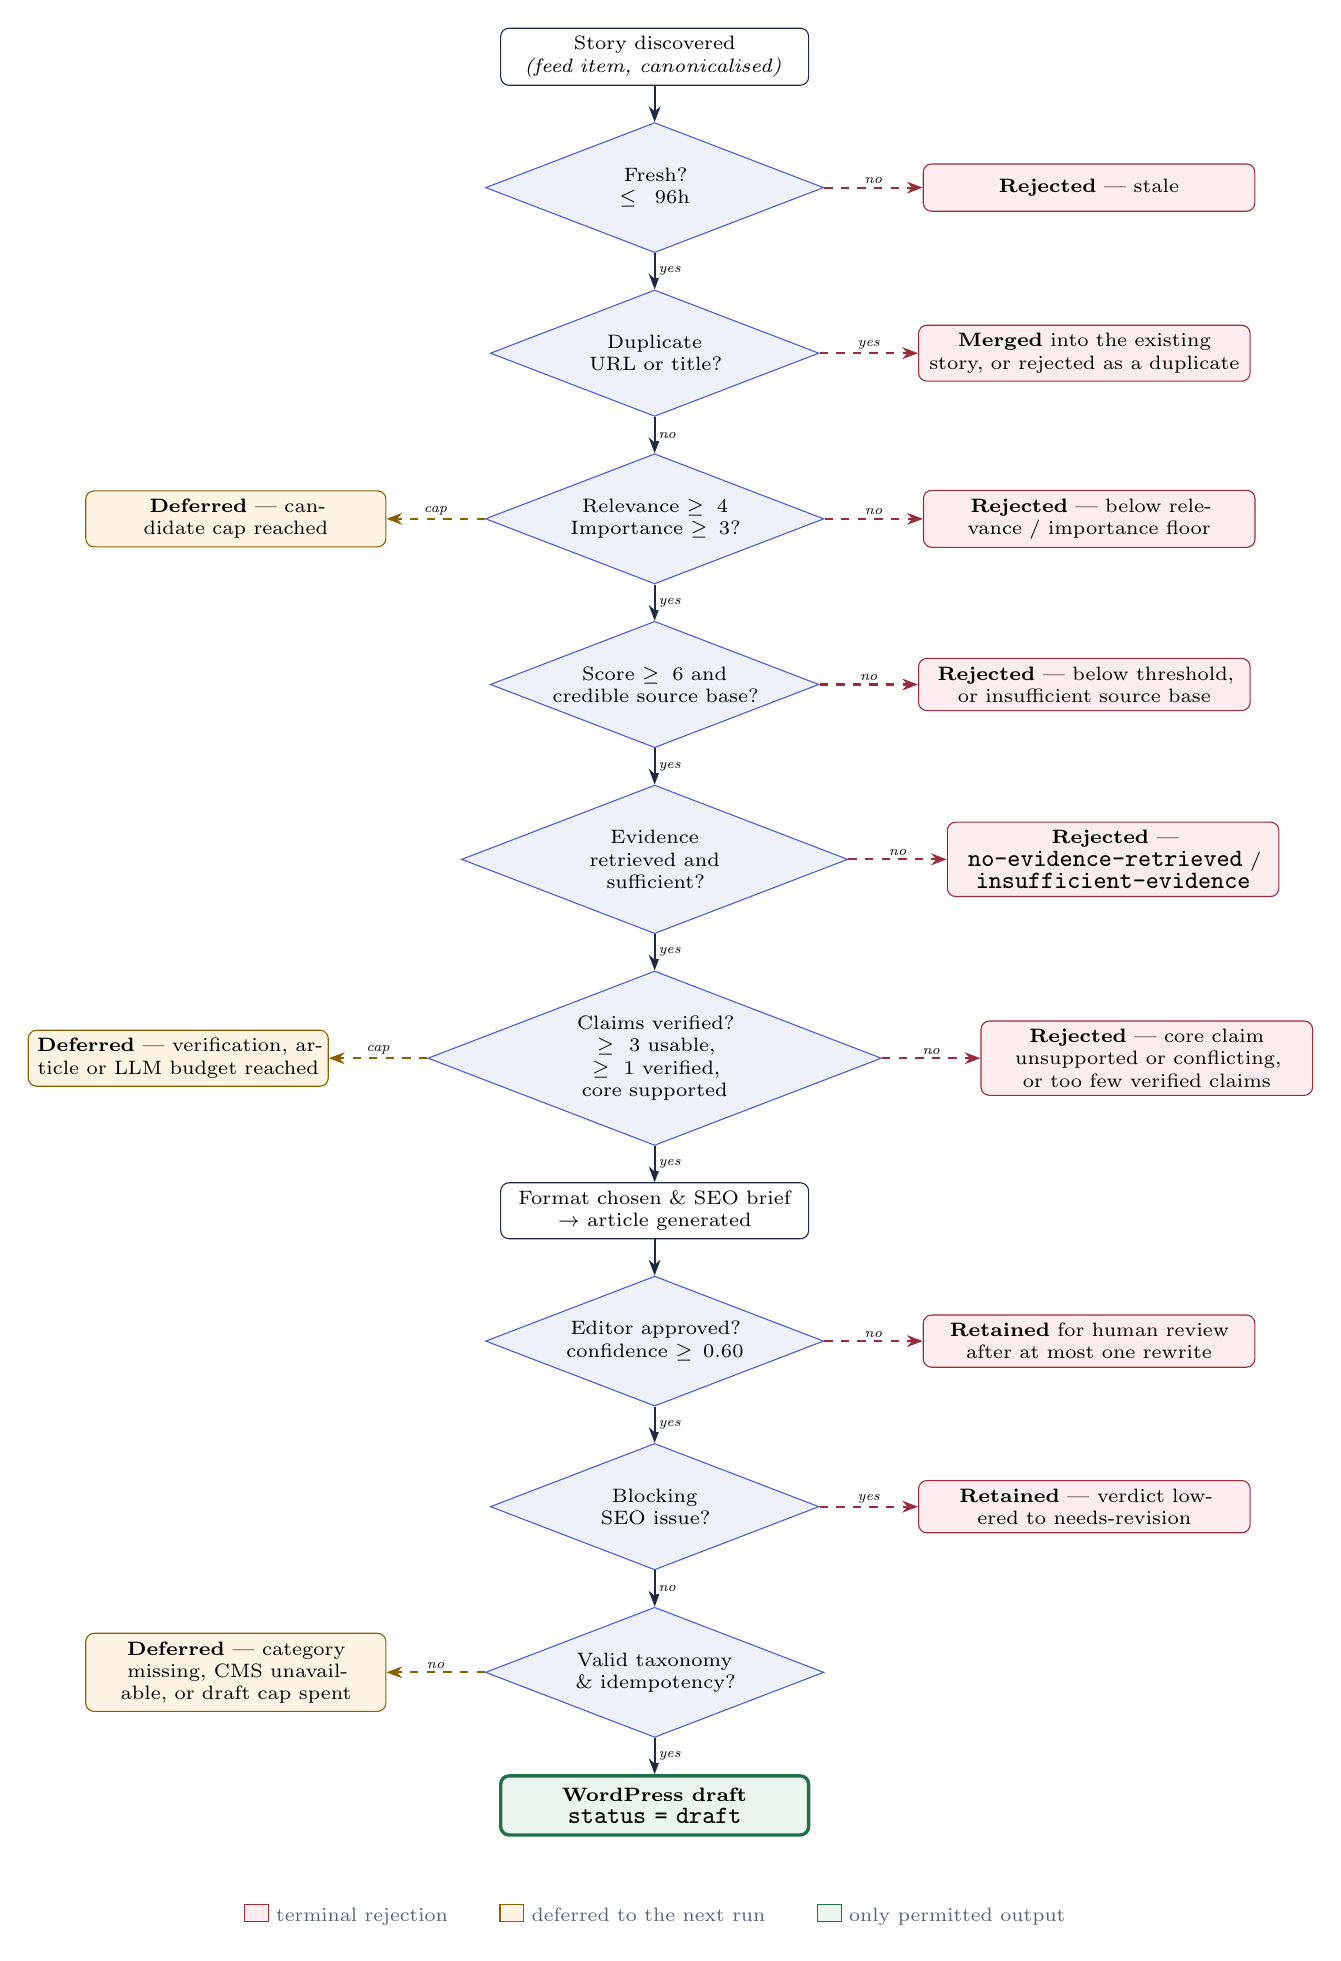
\begin{tikzpicture}[node distance=0.46cm and 1.25cm]
\scriptsize
\tikzset{
  s/.style={rectangle, rounded corners=3pt, draw=aitkNavy, fill=white,
            text width=3.7cm, align=center, minimum height=0.68cm, font=\scriptsize, inner sep=3pt},
  d/.style={diamond, aspect=2.6, draw=aitkAccent, fill=aitkSoft,
            text width=3.0cm, align=center, font=\scriptsize, inner sep=0pt},
  r/.style={rectangle, rounded corners=3pt, draw=aitkStop, fill=aitkStopSoft,
            text width=4.0cm, align=center, minimum height=0.6cm, font=\scriptsize, inner sep=3pt},
  h/.style={rectangle, rounded corners=3pt, draw=aitkHold, fill=aitkHoldSoft,
            text width=3.6cm, align=center, minimum height=0.6cm, font=\scriptsize, inner sep=3pt},
  e/.style={rectangle, rounded corners=3pt, draw=aitkGo, fill=aitkGoSoft, very thick,
            text width=3.7cm, align=center, minimum height=0.75cm, font=\scriptsize\bfseries, inner sep=3pt},
  l/.style={-{Stealth[length=2mm]}, draw=aitkNavy, thick},
  lr/.style={-{Stealth[length=2mm]}, draw=aitkStop, thick, dashed},
  lh/.style={-{Stealth[length=2mm]}, draw=aitkHold, thick, dashed},
  el/.style={font=\tiny\itshape, fill=white, inner sep=1pt}
}

\node[s] (start) {Story discovered\\\textit{(feed item, canonicalised)}};
\node[d, below=of start] (q1) {Fresh?\\$\leq 96$h};
\node[d, below=of q1] (q2) {Duplicate\\URL or title?};
\node[d, below=of q2] (q3) {Relevance $\geq 4$\\Importance $\geq 3$?};
\node[d, below=of q3] (q4) {Score $\geq 6$ and\\credible source base?};
\node[d, below=of q4] (q5) {Evidence\\retrieved and\\sufficient?};
\node[d, below=of q5] (q6) {Claims verified?\\$\geq 3$ usable,\\$\geq 1$ verified,\\core supported};
\node[s, below=of q6] (gen) {Format chosen \& SEO brief\\$\rightarrow$ article generated};
\node[d, below=of gen] (q7) {Editor approved?\\confidence $\geq 0.60$};
\node[d, below=of q7] (q8) {Blocking\\SEO issue?};
\node[d, below=of q8] (q9) {Valid taxonomy\\\& idempotency?};
\node[e, below=of q9] (wp) {WordPress draft\\\code{status = draft}};

% Rejections (right)
\node[r, right=of q1] (r1) {\textbf{Rejected} --- stale};
\node[r, right=of q2] (r2) {\textbf{Merged} into the existing story, or rejected as a duplicate};
\node[r, right=of q3] (r3) {\textbf{Rejected} --- below relevance / importance floor};
\node[r, right=of q4] (r4) {\textbf{Rejected} --- below threshold, or insufficient source base};
\node[r, right=of q5] (r5) {\textbf{Rejected} --- \code{no-evidence-retrieved} / \code{insufficient-evidence}};
\node[r, right=of q6] (r6) {\textbf{Rejected} --- core claim unsupported or conflicting, or too few verified claims};
\node[r, right=of q7] (r7) {\textbf{Retained} for human review after at most one rewrite};
\node[r, right=of q8] (r8) {\textbf{Retained} --- verdict lowered to needs-revision};

% Deferrals (left)
\node[h, left=of q3] (h1) {\textbf{Deferred} --- candidate cap reached};
\node[h, left=of q6] (h2) {\textbf{Deferred} --- verification, article or LLM budget reached};
\node[h, left=of q9] (h3) {\textbf{Deferred} --- category missing, CMS unavailable, or draft cap spent};

% Main spine
\draw[l] (start) -- (q1);
\draw[l] (q1) -- node[el,right]{yes} (q2);
\draw[l] (q2) -- node[el,right]{no} (q3);
\draw[l] (q3) -- node[el,right]{yes} (q4);
\draw[l] (q4) -- node[el,right]{yes} (q5);
\draw[l] (q5) -- node[el,right]{yes} (q6);
\draw[l] (q6) -- node[el,right]{yes} (gen);
\draw[l] (gen) -- (q7);
\draw[l] (q7) -- node[el,right]{yes} (q8);
\draw[l] (q8) -- node[el,right]{no} (q9);
\draw[l] (q9) -- node[el,right]{yes} (wp);

% Rejection edges
\draw[lr] (q1) -- node[el,above]{no} (r1);
\draw[lr] (q2) -- node[el,above]{yes} (r2);
\draw[lr] (q3) -- node[el,above]{no} (r3);
\draw[lr] (q4) -- node[el,above]{no} (r4);
\draw[lr] (q5) -- node[el,above]{no} (r5);
\draw[lr] (q6) -- node[el,above]{no} (r6);
\draw[lr] (q7) -- node[el,above]{no} (r7);
\draw[lr] (q8) -- node[el,above]{yes} (r8);

% Deferral edges
\draw[lh] (q3) -- node[el,above]{cap} (h1);
\draw[lh] (q6) -- node[el,above]{cap} (h2);
\draw[lh] (q9) -- node[el,above]{no} (h3);

% Legend
\node[below=0.75cm of wp, font=\scriptsize, align=center, color=aitkGray] (leg)
 {\tikz\draw[draw=aitkStop,fill=aitkStopSoft] (0,0) rectangle (0.3,0.22);~terminal rejection \qquad
  \tikz\draw[draw=aitkHold,fill=aitkHoldSoft] (0,0) rectangle (0.3,0.22);~deferred to the next run \qquad
  \tikz\draw[draw=aitkGo,fill=aitkGoSoft] (0,0) rectangle (0.3,0.22);~only permitted output};
\end{tikzpicture}}
\captionof{figure}{End-to-end approval flow. Every diamond is a gate that must be
cleared; there is no path to the green terminal that bypasses one.}
\end{center}

\clearpage

% =============================================================================
\section{Decision Matrix}
% =============================================================================

The complete set of gates, in pipeline order. \textbf{Blocking} gates prevent
publication of that story; \textbf{deferral} gates pause it without judging it.

\begin{center}
\footnotesize
\begin{longtable}{@{}c >{\RaggedRight}p{3.9cm} >{\RaggedRight}p{5.0cm} >{\RaggedRight}p{4.3cm}@{}}
\toprule
\textbf{\#} & \textbf{Stage / gate} & \textbf{Pass condition} & \textbf{Failure outcome} \\
\midrule
\endfirsthead
\toprule
\textbf{\#} & \textbf{Stage / gate} & \textbf{Pass condition} & \textbf{Failure outcome} \\
\midrule
\endhead
\multicolumn{4}{@{}l}{\textcolor{aitkStop}{\textbf{BLOCKING GATES}}} \\
\midrule
1 & Automation enabled & \var{AGENT\us ENABLED} is true & Run exits 0 having done nothing \\
2 & Run lock & No other run is active & Run exits 0; note records the holder \\
3 & Source enabled & \code{enabled: true} in the registry & Source is not read at all \\
4 & Banned domain & Item host is not among the 9 banned domains & Dropped at ingestion; \code{banned-domain} \\
5 & Title is a real headline & $\geq 12$ characters & Dropped; \code{title-too-short} \\
6 & URL deduplication & Canonical URL not already persisted & Item dropped as a duplicate \\
7 & Story not terminal & Status is not published or rejected, and it is not a merged duplicate & \code{already-published}, \code{previously-rejected}, \code{duplicate-of-}\allowbreak\code{existing-story} \\
8 & Freshness & Freshest item $\leq 96$ hours old & Rejected; \code{stale (\textit{n}h old)} \\
9 & Hard-rejected topic & No hard-reject keyword rule matches & Rejected; \code{excluded-topic:\textit{id}} \\
10 & Has source items & At least one item backs the story & Rejected; \code{no-source-items} \\
11 & Relevance floor & Classifier relevance $\geq 4$ & Rejected; \code{below-relevance-floor} \\
12 & Importance floor & Classifier importance $\geq 3$ & Rejected; \code{below-importance-floor} \\
13 & Weighted threshold & $S \geq 6.0$ & Rejected; \code{below-threshold} \\
14 & Credible source base & Tier 1 present, or $\geq 2$ independent publishers & Rejected; \code{insufficient-}\allowbreak\code{source-base} \\
15 & Evidence sufficiency & $\geq 1$ Tier 1 document retrieved, or $\geq 2$ distinct Tier 2 publishers & Rejected; \code{no-evidence-retrieved} or \code{insufficient-evidence} \\
16 & Source integrity & No retrieved document attempts prompt injection & Document quarantined; story rejected if sufficiency is lost \\
17 & Claim extraction & At least one atomic claim extracted & Rejected; \code{no-claims-extracted} \\
18 & Core claim support & Core claim is not unsupported, and not conflicting without Tier 1 resolution & Rejected; \code{core-claim-unsupported} / \code{core-claim-conflicting} \\
19 & Verified-claim floor & $\geq 3$ usable claims and $\geq 1$ fully verified & Rejected; \code{too-few-}\allowbreak\code{verified-claims} / \code{no-fully-}\allowbreak\code{verified-claims} \\
20 & Hard word ceiling & Rendered draft $\leq 1400$ words & Draft rejected as runaway output \\
21 & Deterministic editorial checks & Sources section present, source URLs recorded, claim traceability, excerpt $\geq 80$ chars, $\leq 5$ tags, no banned phrase, only allowlisted HTML tags & Verdict forced to \code{needs-revision}; draft retained, never sent \\
22 & Editorial verdict & Model returns \code{approved} with no blocking issue & Retained; \code{editorial:}\allowbreak\code{needs-revision} or \code{editorial:rejected} \\
23 & Confidence floor & Editorial confidence $\geq 0.60$ & Verdict lowered to \code{needs-revision}; \code{low-confidence} \\
24 & SEO blocking findings & No blocking SEO issue & Approved verdict lowered to \code{needs-revision} \\
25 & Publication idempotency & No existing \code{wp\_post\_id}; story is not a duplicate of a published one & Skipped; \code{already-published} or \code{duplicate-of-}\allowbreak\code{published-story} \\
\midrule
\multicolumn{4}{@{}l}{\textcolor{aitkHold}{\textbf{DEFERRAL GATES} --- the story survives and is reconsidered next run}} \\
\midrule
D1 & Candidate cap & Fewer than 20 stories classified this run & \code{candidate-}\allowbreak\code{budget-reached} \\
D2 & Verification cap & Fewer than 5 stories verified this run & \code{verification-}\allowbreak\code{budget-reached} \\
D3 & Article cap & Fewer than 2 articles written this run & \code{article-budget-reached} \\
D4 & Model budget & Call and token budgets not exhausted & \code{llm-budget-exhausted} \\
D5 & Draft cap & Fewer than 2 posts created this run & Approved article stays pending \\
D6 & Category exists in CMS & Category is present in WordPress & \code{category-not-configured} \\
D7 & CMS reachable & WordPress responds & \code{wordpress-unavailable} / \code{wordpress-}\allowbreak\code{not-configured} \\
\bottomrule
\end{longtable}
\end{center}

\begin{center}
\small
\begin{tabularx}{\textwidth}{@{}l c >{\RaggedRight}X@{}}
\toprule
\textbf{Category} & \textbf{Count} & \textbf{Effect} \\
\midrule
Blocking gates & \textbf{25} & Failure prevents publication of that story \\
Deferral gates & \textbf{7} & Failure pauses the story without judging it \\
\bottomrule
\end{tabularx}
\end{center}

% =============================================================================
\section{Examples}
% =============================================================================

The three walkthroughs below describe how the implemented pipeline behaves in
each of its three outcomes. Story details are illustrative; every threshold,
reason code and behaviour quoted is the real one.

\subsection{Example A --- Accepted}

\begin{center}
\small
\begin{tabularx}{\textwidth}{@{}p{3.9cm} >{\RaggedRight}X@{}}
\toprule
\textbf{Stage} & \textbf{What happens} \\
\midrule
Discovery & A vendor's official blog (Tier 1) and two technology publications
  (Tier 2) each publish on the same capability change. Four items arrive across
  three feeds. \\
Deduplication & Canonical URLs differ, so no item is dropped at level 1/2. Title
  similarity is above 0.62 and the headlines share two distinctive tokens, so all
  four items cluster into \textbf{one story} from three independent publishers. \\
Freshness \& rules & Freshest item is 5 hours old (within 96). No banned domain, no
  hard-rejected topic. Included-topic rules match \code{model-update} and
  \code{capability}; two audience entities are named. \\
Scoring & Classifier returns $R=8$, $I=7$. Trust: best tier 1 gives 10, plus 2
  corroboration points, capped at 10. Freshness at 5 hours $\approx 9.5$.
  $S_{\text{base}} = 0.35(8)+0.30(7)+0.20(10)+0.15(9.5) = 8.33$; the topic prior
  adds the clamped maximum $+2$, so $S = 10.0$ after clamping. \\
Selection & Clears all four gates: $R \geq 4$, $I \geq 3$, $S \geq 6$, Tier 1
  present. \textcolor{aitkGo}{\textbf{Selected}}, and sorted first by score. \\
Evidence & Tier 1 fetched first, then the two Tier 2 pages; the fourth is beyond
  the 4-page budget. Three documents retrieved, all above the 200-character floor,
  none flagged for injection. Tier 1 present $\Rightarrow$ \textbf{sufficient}. \\
Claims & Extraction runs once per document. Overlapping claims merge, leaving
  \textbf{14 distinct claims} across types \code{launch}, \code{capability},
  \code{pricing} and \code{date}. \\
Verification & The core \code{launch} claim is confirmed by Tier 1 and both Tier 2
  publishers $\Rightarrow$ \code{verified}. \code{capability} and \code{pricing}
  claims are backed by Tier 1 $\Rightarrow$ \code{verified}. Two claims appear only
  in one publication $\Rightarrow$ \code{single-source}. Result: \textbf{9 verified,
  2 single-source}. Passes all four story-level gates. \\
Format & 9 verified claims, 3 sources, 3 publishers $\Rightarrow$ meets
  \code{standard} but not \code{analysis} (needs 12 claims and importance $\geq 7$
  --- importance qualifies, claim count does not). \textbf{Format: standard,
  500--900 words}. \\
SEO brief & Grounded primary keyword, 4 secondary keywords, a 148-character meta
  description, a normalised slug, and one internal link chosen from the route
  allowlist. \\
Writing & 11 usable claims supplied; the 3 unsupported ones are withheld entirely.
  The two single-source claims are attributed in the prose. Draft comes in at 690
  words across 6 sections. \\
Editorial & No unsupported statements, headline matches the body, attribution
  present, no banned phrase, 4 entity tags, only allowlisted HTML, Sources section
  rendered. Confidence \textbf{0.82} $\geq 0.60$. \textbf{Verdict:
  \code{approved}.} \\
SEO validation & No blocking findings; one advisory
  (\code{seo-keyword-not-in-heading}). Verdict unchanged. \\
Publication & Category on the allowlist and present in WordPress; 4 tags resolved
  (one created); no existing post identifier; draft budget available. \\
\midrule
\textbf{Outcome} & \textcolor{aitkGo}{\textbf{WordPress draft created,
  \code{status = draft}}}, awaiting human review. \\
\bottomrule
\end{tabularx}
\end{center}

\subsection{Example B --- Rejected}

\begin{center}
\small
\begin{tabularx}{\textwidth}{@{}p{3.9cm} >{\RaggedRight}X@{}}
\toprule
\textbf{Stage} & \textbf{What happens} \\
\midrule
Discovery & A single Tier 1 vendor feed carries a strong, specific headline about
  a major capability change. One item, one publisher. \\
Freshness \& rules & 3 hours old. No banned domain, no hard-rejected topic.
  Included-topic rules match strongly. \\
Scoring & Classifier returns $R=9$, $I=8$ from the headline and feed summary.
  Trust $= 10$ (Tier 1, no corroboration bonus). Freshness $\approx 9.7$.
  $S = 9.1$ --- comfortably above the threshold. \\
Selection & Passes: $R$ and $I$ clear their floors, $S \geq 6$, and the source-base
  gate is satisfied because a Tier 1 source is present.
  \textcolor{aitkGo}{\textbf{Selected}} --- at this point the story looks excellent. \\
Evidence & The agent fetches the article URL. The publisher returns
  \textbf{HTTP 403}. As a 4xx it is \textbf{not retried}; the fetch is counted as
  failed and contributes no evidence. No other item backs the story, so there is
  nothing else to fetch. \\
Sufficiency & Zero documents retrieved.
  $\Rightarrow$ \textbf{insufficient}. \\
\midrule
\textbf{Outcome} & \textcolor{aitkStop}{\textbf{Rejected}}, reason
  \code{no-evidence-retrieved}. The story is marked with evidence state
  \code{insufficient}, the reason is persisted, and \textbf{no model call is made
  beyond the classifier}. \\
\bottomrule
\end{tabularx}
\end{center}

\begin{blockbox}[Why this is the correct outcome]
The agent had a trusted publisher, a high score, and a headline specific enough to
write from. It still produced nothing, because it could not read the document. A
system willing to write from a headline would have produced a confident, plausible,
\emph{unverified} article here --- which is exactly the failure this pipeline is
built to make impossible. Had a second independent publisher also covered the
story and been reachable, evidence sufficiency would have been met by two Tier 2
publishers and the story would have continued, with capability and pricing claims
downgraded to \code{single-source} and attributed.
\end{blockbox}

\subsection{Example C --- Deferred}

\begin{center}
\small
\begin{tabularx}{\textwidth}{@{}p{3.9cm} >{\RaggedRight}X@{}}
\toprule
\textbf{Stage} & \textbf{What happens} \\
\midrule
Context & A busy run. Two higher-scoring stories have already been written, and
  \var{AGENT\us MAX\us ARTICLES\us PER\us RUN} is at its default of \textbf{2}. \\
This story & A legitimate, well-sourced launch scoring $S = 7.4$: Tier 1 present,
  fresh, relevant. It clears every selection gate and is
  \textcolor{aitkGo}{\textbf{selected}}, but sorts third by weighted score. \\
The cap & On reaching it, the loop finds
  \code{articlesGenerated (2) $\geq$ maxArticles (2)}. \\
Action taken & The story is set to \code{deferred} with reason
  \code{article-budget-reached}. The run's deferred counter increments. \textbf{No
  evidence is gathered, no claims extracted, no model budget spent on it.} \\
Next run & Deferred stories are loaded \emph{first} and queued \textbf{ahead of}
  newly discovered candidates, because they already carry a score. This story is
  re-checked by the prefilter against the current clock. \\
If still fresh & It proceeds through evidence, verification, writing and review
  exactly as any other story would. \\
If now stale & Having aged past 96 hours, it is \textcolor{aitkStop}{rejected} with
  \code{stale (\textit{n}h old)} rather than lingering as a permanent backlog
  entry. \\
\midrule
\textbf{Outcome} & \textcolor{aitkHold}{\textbf{Deferred}} --- a statement about the
  run's budget, not about the story's quality. \\
\bottomrule
\end{tabularx}
\end{center}

\begin{infobox}[The same behaviour at every cap]
Identical logic applies at each of the five budget boundaries. The candidate cap
defers before classification; the verification cap defers before evidence
gathering; the article cap defers before writing; model call and token budgets
defer at whatever point they are reached; and the draft cap leaves an
\emph{already-approved} article pending, to be posted by the next run at no model
cost. In every case the reason is recorded and the story keeps its place.
\end{infobox}

% =============================================================================
\section{What the LLM Does vs What Code Decides}
% =============================================================================

This division is the core of the system's trustworthiness. The model contributes
judgement; code contributes authority.

\begin{center}
\small
\begin{tabularx}{\textwidth}{@{}>{\RaggedRight}p{5.3cm} >{\RaggedRight}X@{}}
\toprule
\textcolor{aitkAccent}{\textbf{Decided by the model}} & \textbf{And how code constrains it} \\
\midrule
Semantic relevance and importance (0--10) & Clamped to range, combined with
  code-computed trust and freshness under fixed weights, then checked against
  independent floors the model cannot see or influence. \\
Novelty score & \textbf{Not consumed.} Produced and validated, read by nothing. \\
Editorial category & Constrained to a closed enumeration of 10; anything
  unrecognised falls back to \code{industry}. \\
Recommendation (\code{proceed}/\code{skip}) & \textbf{Advisory only.} Logged and
  displayed; never decisive. \\
Claim extraction & Bounded to 25 claims per source, one source per call, closed
  type enumeration, strict schema. Instruction-shaped claims are dropped by code.
  Support level is not set here. \\
Claim verification & Supporting URLs are filtered to the story's real evidence set;
  tier rules then \textbf{downgrade} any verdict the evidence does not justify;
  ignored claims default to unsupported. The rules never upgrade. \\
Article prose & Receives only verified and single-source claims --- never source
  documents. Returns structured sections, never markup. Hard word ceiling enforced
  by code. \\
Editorial review & Its \code{approved} verdict is overridden by any deterministic
  blocking issue and by a confidence below 0.60. If the review cannot run, the
  draft is rejected, not waved through. \\
SEO brief & Every field is re-checked against the verified claims by code. The
  slug is re-derived. Internal links are filtered against a route allowlist. \\
\bottomrule
\end{tabularx}
\end{center}

\begin{center}
\small
\begin{tabularx}{\textwidth}{@{}>{\RaggedRight}p{5.3cm} >{\RaggedRight}X@{}}
\toprule
\textcolor{aitkGo}{\textbf{Decided by deterministic code}} & \textbf{Implementation} \\
\midrule
Source enablement and tiering & Static registry; the model never sees a feed list
  or chooses a source. \\
Freshness & Arithmetic on timestamps against a 96-hour window. \\
Duplicate detection & URL canonicalisation, database uniqueness constraint, and
  token/bigram title similarity with fixed thresholds. \\
Threshold enforcement & Relevance, importance, weighted score and source-base gates
  --- all applied after the model has answered, to values it cannot revise. \\
Cost caps & Call and token budgets, per-stage caps, enforced by a circuit breaker
  that throws before a call is made. \\
Article format and length band & Computed from verified-claim and publisher counts.
  Explicitly not a model call, so the model cannot argue for a longer article. \\
Category allowlist & Ten fixed terms; never created during publishing. \\
Tag validation and count & Character class, length, word count, markup, control
  characters, theme-vs-entity shape, presence in the article, slug deduplication,
  maximum of 5. \\
HTML safety & Fixed tag allowlist, unconditional escaping, validated link targets.
  The model never supplies markup. \\
Slug generation & Deterministic from the title; stable across revisions and
  retries. \\
Draft-only policy & Hardcoded in the payload, asserted again at the HTTP boundary,
  with startup refusing an auto-publish configuration. \\
Idempotency & Three publication guards plus an immediate, non-overwritable
  database write of the post identifier. \\
Network safety & HTTPS-only, SSRF address checks, response size caps, timeouts,
  bounded redirects. \\
Secret handling & Credentials registered for redaction; a test asserts no
  credential appears in logs even at debug level. \\
\bottomrule
\end{tabularx}
\end{center}

\begin{blockbox}[The model has no publishing authority]
At no point does a model decide that something is published. It cannot enable a
source, raise its own score past a threshold, extend its own word budget, create a
category, emit markup, set a URL, choose a post status, or call the CMS. Its most
favourable possible output is a \emph{recommendation} that deterministic code then
accepts or refuses. Conversely, a model verdict of ``reject'' is always honoured:
the asymmetry runs one way only.
\end{blockbox}

% =============================================================================
\section{Limitations}
% =============================================================================

Stated plainly, because a system whose limits are known is easier to operate than
one whose limits are discovered.

\subsection{Source access}

\begin{itemize}[leftmargin=1.2em,itemsep=0.25em]
  \item \textbf{Blocked source URLs.} Some publishers return HTTP 403 to automated
    readers. Those documents contribute no evidence and, if the story depends on
    them, it is rejected. This is a correct outcome but a real coverage loss.
  \item \textbf{Paywalls, consent walls and JavaScript shells.} A page yielding
    under 200 characters of extractable text is discarded. No headless browser is
    used, deliberately.
  \item \textbf{Six Tier 1 vendors are currently unreachable.} Anthropic, Meta AI,
    Mistral, Microsoft, Runway --- and Ars Technica at Tier 2 --- publish no stable
    feed the agent can use. They are registered as disabled with the reason
    recorded, rather than pointed at a guessed URL that would fail silently. News
    from those vendors is therefore only picked up when a configured Tier 2
    publication covers it.
  \item \textbf{No Tier 3 sources are configured.} Tier 3 exists in the trust model
    and is the default assigned to unrecognised hosts, but nothing currently feeds
    it, so its behaviour is exercised only by tests.
  \item \textbf{Article-text extraction is heuristic.} Boilerplate removal is
    pattern-based; a wrong guess degrades text quality rather than creating a
    safety issue, since the output is plain text either way.
  \item \textbf{Publisher independence is approximated} by registrable domain,
    without a public-suffix list. Occasional mistakes on multi-part country domains
    are possible and harmless.
\end{itemize}

\subsection{Model and API availability}

\begin{itemize}[leftmargin=1.2em,itemsep=0.25em]
  \item A provider outage, an exhausted credit balance or a rejected key stops the
    run rather than degrading quality --- an invalid credential fails identically for
    every story, so it aborts instead of rejecting the whole queue one call at a
    time.
  \item Structured-output failures get one repair pass and one clean retry
    (3 attempts). Persistently invalid output is rejected, never accepted.
  \item A model refusal surfaces as a refusal, never as article content.
  \item The editorial pass failing means \emph{rejection}, not approval.
    Availability problems therefore cost articles, never quality.
\end{itemize}

\subsection{Evidence and coverage}

\begin{itemize}[leftmargin=1.2em,itemsep=0.25em]
  \item At most \textbf{4} evidence pages per story, and no links are followed out
    of fetched pages. The agent cannot go looking for corroboration that its own
    feeds did not surface.
  \item A legitimate article \emph{about} prompt injection will be quarantined by
    the injection detector. This false positive is accepted deliberately: losing a
    meta-story is cheaper than republishing manipulated content, and the rejection
    is logged for a human to overturn.
  \item Deduplication may occasionally merge two genuinely distinct stories. The
    bias toward merging is deliberate --- a wrong merge loses one article, a wrong
    split publishes a duplicate.
\end{itemize}

\subsection{Article shape}

\begin{itemize}[leftmargin=1.2em,itemsep=0.25em]
  \item \textbf{Thin stories produce short briefs}, by design. A 180--350 word
    article where every sentence is grounded is a success, not a shortfall. Clients
    reviewing output should expect briefs to be common.
  \item The \code{analysis} format requires 12 verified claims, 3 sources, 3
    publishers \emph{and} importance $\geq 7$, so it will be rare.
  \item The optional editorial ``AI Tool Kart take'' section described in the design
    brief is not implemented; the writer is given five factual headings only.
\end{itemize}

\subsection{SEO metadata}

\begin{holdbox}[The SEO brief is stored locally, not written to the CMS]
The production site runs All in One SEO, which was inspected before this layer was
built. It offers no safe write path for the agent: its fields appear on reads but
are absent from the writable post schema, its own save route is an undocumented
internal endpoint, and the agent's least-privilege role receives HTTP 403 from its
options endpoint. Writing SEO fields would mean reverse-engineering an
undocumented endpoint \emph{and} raising the agent's CMS privileges --- both poor
trades for metadata a human can set in seconds during review.

So the brief is persisted with the article and surfaced to the reviewer, and the
CMS sink is a deliberate no-op behind a one-file interface. What does still reach
the site is the title and the excerpt --- which matters, because the plugin's stock
description template is the post excerpt, so a well-written excerpt commonly becomes
the rendered meta description with no plugin API at all.
\end{holdbox}

\subsection{Featured images}

No featured image is ever attached. The field is absent from the post payload
entirely, and a test asserts it. The front end already renders a gradient fallback
in the same frame when an image is missing, so the grid stays on its baseline.
Automatic image generation is an explicit non-goal at this stage.

\subsection{Human review remains required}

\begin{blockbox}[Nothing reaches a reader without a person]
The agent's output is a WordPress draft. Publication is a human action. Every gate
in this document reduces the volume and raises the floor of what a reviewer sees;
none of them replaces the reviewer. The draft carries everything needed to check it
without leaving the editor: the rendered Sources block, the claim identifiers used,
the editorial verdict, confidence score and full issue list, the assigned format
and its target range, and the SEO brief.
\end{blockbox}

% =============================================================================
\section{Conclusion}
% =============================================================================

Whether a story becomes an article is not a single judgement. It is the product of
eight independent layers, each of which can stop the story on its own:

\begin{center}
\small
\begin{tabularx}{\textwidth}{@{}p{4.3cm} >{\RaggedRight}X@{}}
\toprule
\textbf{Layer} & \textbf{Contribution} \\
\midrule
Deterministic filters & Source enablement, banned domains, title validity,
  freshness, URL and title deduplication, hard-rejected topics --- all free, all
  before any model call. \\
Weighted scoring & Four dimensions under fixed weights, with independent relevance,
  importance, score and source-base floors. \\
Evidence quality & Documents must be \emph{retrieved}, not merely referenced, and
  must meet a tier-based sufficiency rule. \\
Fact verification & Per-claim support levels, with deterministic tier rules that
  only ever downgrade, and four story-level gates. \\
Editorial review & An independent pass against the same claims, with code
  overriding an over-generous verdict and a bounded single revision. \\
SEO review & Grounding, superlative and stuffing checks that can lower a verdict
  but never raise one. \\
Taxonomy validation & A fixed category allowlist never extended at publish time,
  and a validated entity-tag vocabulary. \\
Budget and safety controls & Per-run caps that defer rather than reject, HTML and
  URL safety boundaries, idempotency guards, and a draft-only publishing policy. \\
\bottomrule
\end{tabularx}
\end{center}

\vspace{0.5em}

\begin{gobox}[The design preference, stated once more]
\begin{center}
\large
\textbf{no article} \quad is always preferred to \quad \textbf{unsupported article}
\end{center}
\vspace{0.2em}
Every ambiguous case in this pipeline resolves toward not publishing. Evidence that
cannot be retrieved ends the story. A claim the sources do not establish is removed
rather than softened. A review that cannot run is a rejection, not a pass. A budget
that runs out pauses work rather than lowering the bar. And the most favourable
outcome the system can produce on its own is a draft, waiting for a person to
decide.
\end{gobox}

\vspace{0.6em}

{\footnotesize\color{aitkGray}
This behaviour is not merely intended; it is asserted. The agent's test suite
covers the selection thresholds, the tier downgrade rules, the format decision, the
dedupe thresholds, the revision bound, the SEO monotonicity rule, the tag and
category validation, the HTML allowlist, the injection quarantine, the draft-only
policy, the idempotency guards, the cap semantics including the fail-closed zero
case, and the pending-publication retry. All \textbf{422} tests pass at the time of
writing.\par}

\clearpage
\appendix
\renewcommand{\thesection}{\Alph{section}}
\titleformat{\section}
  {\normalfont\Large\bfseries\color{aitkNavy}}{Appendix \thesection.}{0.7em}{}

% =============================================================================
\section{Current Configurable Parameters}
\label{app:params}
% =============================================================================

Every parameter below materially affects story selection, article approval, or
publication. Environment variables are shown with their documented defaults; code
constants are shown with their current values and the file that owns them.

\begin{blockbox}[No credentials appear in this document]
\var{LLM\us API\us KEY}, \var{WORDPRESS\us USERNAME} and
\var{WORDPRESS\us APP\us PASSWORD} are listed by \emph{name and purpose only}.
Their values are never printed here, never logged by the agent (secrets are
registered for redaction at startup, and a test asserts no credential appears even
at debug level), and never exposed to the browser bundle.
\end{blockbox}

\subsection{Environment variables (25)}

\begin{center}
\footnotesize
\begin{longtable}{@{}>{\RaggedRight}p{5.4cm} >{\RaggedRight}p{6.2cm} >{\RaggedRight}p{3.5cm}@{}}
\toprule
\textbf{Variable} & \textbf{Purpose} & \textbf{Default} \\
\midrule
\endfirsthead
\toprule
\textbf{Variable} & \textbf{Purpose} & \textbf{Default} \\
\midrule
\endhead
\var{LLM\us PROVIDER} & Which model provider to use; \code{mock} runs the pipeline
  offline with a deterministic provider & \code{mock} \\
\var{LLM\us API\us KEY} & Provider credential. Required for any non-mock provider;
  the agent refuses to start without one & \textit{(not set)} \\
\var{LLM\us MODEL\us FAST} & Override for the cheap model class (classification,
  extraction, SEO) & adapter default \\
\var{LLM\us MODEL\us STRONG} & Override for the strong model class (verification,
  writing, editing) & adapter default \\
\var{WORDPRESS\us API\us URL} & CMS REST base including namespace. HTTPS required
  except for loopback/\code{.local} development hosts & \textit{(not set)} \\
\var{WORDPRESS\us USERNAME} & Dedicated least-privilege CMS account (not an
  administrator) & \textit{(not set)} \\
\var{WORDPRESS\us APP\us PASSWORD} & CMS application password & \textit{(not set)} \\
\var{WORDPRESS\us CREATE\us TERMS} & Whether missing \textbf{tags} may be created.
  Categories are never created regardless & \code{true} \\
\var{AGENT\us DB\us PATH} & SQLite database path (dedupe, idempotency, audit trail)
  & \code{./data/}\allowbreak\code{news-agent.sqlite} \\
\var{AGENT\us ENABLED} & Automation kill switch. False exits cleanly before the
  database, provider or network are touched & \code{true} \\
\var{AGENT\us AUTO\us PUBLISH} & Must be false. True causes startup to
  \textbf{fail}; no code path could honour it & \code{false} \\
\var{AGENT\us MAX\us ITEMS\us PER\us SOURCE\us PER\us RUN} & Items taken from any one
  feed per run & \code{25} \\
\var{AGENT\us MAX\us CANDIDATES\us PER\us RUN} & Stories sent to the relevance
  classifier & \code{20} \\
\var{AGENT\us MAX\us STORIES\us VERIFIED\us PER\us RUN} & Stories taken through
  evidence, extraction and verification & \code{5} \\
\var{AGENT\us MAX\us ARTICLES\us PER\us RUN} & Articles written per run & \code{2} \\
\var{AGENT\us MAX\us DRAFTS\us PER\us RUN} & Total CMS posts per run, retries
  included & \code{2} \\
\var{AGENT\us MAX\us LLM\us CALLS\us PER\us RUN} & Absolute circuit breaker on model
  calls & \code{60} \\
\var{AGENT\us MAX\us TOKENS\us PER\us RUN} & Absolute circuit breaker on tokens &
  \code{250000} \\
\var{AGENT\us MIN\us WEIGHTED\us SCORE} & Weighted score (0--10) a story must reach
  to earn evidence gathering & \code{6} \\
\var{AGENT\us HTTP\us TIMEOUT\us MS} & Per-request timeout for feeds and evidence &
  \code{15000} \\
\var{AGENT\us MAX\us RESPONSE\us BYTES} & Response size cap & \code{2500000} \\
\var{AGENT\us USER\us AGENT} & Identifying user agent sent to publishers &
  \code{AIToolKart}\allowbreak\code{NewsAgent/0.1} \\
\var{AGENT\us RUN\us LOCK\us STALE\us MINUTES} & Age at which a run lock is
  reclaimed & \code{30} \\
\var{AGENT\us LOG\us FORMAT} & \code{json} for production, \code{pretty} for humans
  & \code{pretty} \\
\var{AGENT\us LOG\us LEVEL} & Log verbosity & \code{info} \\
\bottomrule
\end{longtable}
\end{center}

\subsection{Scoring and selection constants (12)}

\begin{center}
\footnotesize
\begin{tabularx}{\textwidth}{@{}>{\RaggedRight}p{5.0cm} c >{\RaggedRight}X@{}}
\toprule
\textbf{Constant} & \textbf{Value} & \textbf{Purpose} \\
\midrule
\code{SCORE\_WEIGHTS.relevance} & 0.35 & Weight on classifier relevance \\
\code{SCORE\_WEIGHTS.importance} & 0.30 & Weight on classifier importance \\
\code{SCORE\_WEIGHTS.sourceTrust} & 0.20 & Weight on computed source trust \\
\code{SCORE\_WEIGHTS.freshness} & 0.15 & Weight on computed freshness \\
\code{TIER\_TRUST\_SCORE} & 10 / 7 / 3 & Trust contributed by Tier 1 / 2 / 3 \\
\code{CORROBORATION\_BONUS} & 1 & Points per additional independent publisher \\
\code{MAX\_CORROBORATION\_BONUS} & 2 & Ceiling, so rewrites cannot outrank a primary source \\
\code{FRESHNESS\_HALF\_LIFE\_HOURS} & 48 & Freshness decays linearly to zero over twice this \\
\code{MIN\_RELEVANCE} & 4 & Hard relevance floor, independent of the score \\
\code{MIN\_IMPORTANCE} & 3 & Hard importance floor \\
Topic-prior clamp & $\pm 2$ & Limit on how far keyword rules may move a score \\
Entity-bonus cap & $3 \times 0.5$ & Limit on audience-entity contribution \\
\bottomrule
\end{tabularx}
\end{center}
\technote{\file{src/config/limits.ts}, \file{src/ranking/score.ts}, \file{src/ranking/prefilter.ts}.}

\subsection{Deduplication and freshness (6)}

\begin{center}
\footnotesize
\begin{tabularx}{\textwidth}{@{}>{\RaggedRight}p{5.0cm} c >{\RaggedRight}X@{}}
\toprule
\textbf{Constant} & \textbf{Value} & \textbf{Purpose} \\
\midrule
\code{DEDUPE.sameStoryThreshold} & 0.62 & Title similarity at or above this is one story \\
\code{DEDUPE.ambiguousThreshold} & 0.50 & Merge but flag; same-publisher guard applies \\
\code{DEDUPE.clusterWindowHours} & 72 & Titles only cluster within this window \\
\code{maxStoryAgeHours} & 96 & Staleness gate, measured from the freshest item \\
\code{minTitleLength} & 12 & Below this a title is a stub, not a story \\
\code{MAX\_SLUG\_LENGTH} & 72 & Slug ceiling, truncated on a word boundary \\
\bottomrule
\end{tabularx}
\end{center}

\subsection{Evidence and verification (8)}

\begin{center}
\footnotesize
\begin{tabularx}{\textwidth}{@{}>{\RaggedRight}p{5.0cm} c >{\RaggedRight}X@{}}
\toprule
\textbf{Constant} & \textbf{Value} & \textbf{Purpose} \\
\midrule
\code{MAX\_EVIDENCE\_}\allowbreak\code{FETCHES\_PER\_STORY} & 4 & Evidence pages fetched per story \\
\code{MAX\_EVIDENCE\_CHARS} & 24{,}000 & Cleaned text retained per source \\
Minimum extracted text & 200 chars & Below this a page is a paywall or JS shell \\
\code{MAX\_CLAIMS\_SENT} & 25 & Claims sent to the verifier per story \\
\code{EVIDENCE\_EXCERPT\_CHARS} & 6{,}000 & Evidence excerpt length in the verifier prompt \\
\code{MIN\_VERIFIED\_CLAIMS} & 3 & Usable claims required before writing \\
\code{CLAIM\_RULES} & 8 typed rules & Per-claim-type tier requirements (Section~7) \\
\code{DEFAULT\_CLAIM\_RULE} & 1 Tier 2 & Fallback for an unrecognised claim type \\
\bottomrule
\end{tabularx}
\end{center}

\subsection{Article and editorial constraints (15)}

\begin{center}
\footnotesize
\begin{tabularx}{\textwidth}{@{}>{\RaggedRight}p{5.0cm} >{\RaggedRight}p{3.6cm} >{\RaggedRight}X@{}}
\toprule
\textbf{Constant} & \textbf{Value} & \textbf{Purpose} \\
\midrule
\code{ARTICLE\_FORMATS.brief} & 180--350 words, 3--5 sections & Floor format \\
\code{ARTICLE\_FORMATS.standard} & 500--900 words, 4--7 sections & Common case \\
\code{ARTICLE\_FORMATS.analysis} & 900--1400 words, 5--9 sections & Only when evidence carries it \\
\code{DEFAULT\_ARTICLE\_FORMAT} & \code{standard} & Fallback for pre-format records \\
\code{FORMAT\_THRESHOLDS.standard} & 6 claims / 2 sources / 2 publishers & Bar for \code{standard} \\
\code{FORMAT\_THRESHOLDS.analysis} & 12 claims / 3 sources / 3 publishers / importance 7 & Bar for \code{analysis} \\
\code{ARTICLE.hardMaxWords} & 1400 & Runaway-output rejection ceiling \\
\code{ARTICLE.minTags} & 2 & Advisory tag floor \\
\code{ARTICLE.maxTags} & 5 & Blocking tag ceiling \\
\code{ARTICLE.excerptMinChars} & 80 & Blocking excerpt floor \\
\code{ARTICLE.excerptMaxChars} & 320 & Excerpt ceiling \\
\code{ARTICLE.titleMaxChars} & 110 & Title ceiling \\
\code{MAX\_REVISION\_ATTEMPTS} & 1 & Bounded writer/editor loop \\
\code{MIN\_APPROVAL\_CONFIDENCE} & 0.60 & Editorial confidence floor for approval \\
\code{ALLOWED\_TAGS} & 11 HTML tags & Renderer allowlist: \code{p, h2, h3, ul, ol, li, a, strong, em, blockquote, code} \\
\bottomrule
\end{tabularx}
\end{center}

\subsection{SEO constraints (11)}

\begin{center}
\footnotesize
\begin{tabularx}{\textwidth}{@{}>{\RaggedRight}p{5.0cm} >{\RaggedRight}p{3.6cm} >{\RaggedRight}X@{}}
\toprule
\textbf{Constant} & \textbf{Value} & \textbf{Purpose} \\
\midrule
\code{SEO.metaDescriptionMinChars} & 50 & Below this is not a description \\
\code{SEO.metaDescriptionMaxChars} & 160 & Truncation point in search results \\
\code{SEO.seoTitleMaxChars} & 60 & Soft target; beyond it, advisory warning \\
\code{SEO.seoTitleHardMaxChars} & 80 & Schema ceiling \\
\code{SEO.maxSecondaryKeywords} & 6 & Schema ceiling \\
\code{SEO.maxSuggestedHeadings} & 8 & Schema ceiling \\
\code{SEO.maxInternalLinks} & 4 & Schema ceiling \\
\code{SEO.}\allowbreak\code{maxPrimaryKeywordRepeats} & 4 & Stuffing threshold (a count, not a density) \\
\code{SEO\_BY\_FORMAT} & 3 / 6 / 8 headings; 2 / 4 / 6 keywords; 2 / 3 / 4 links & Per-format shape, so SEO cannot become padding \\
\code{UNSUPPORTED\_SUPERLATIVES} & 24 terms & Ranking words blocked unless verified \\
\code{STATIC\_ROUTES} & 5 routes & Internal-link allowlist, plus this agent's own published slugs \\
\bottomrule
\end{tabularx}
\end{center}

\subsection{Taxonomy and tags (6)}

\begin{center}
\footnotesize
\begin{tabularx}{\textwidth}{@{}>{\RaggedRight}p{5.0cm} c >{\RaggedRight}X@{}}
\toprule
\textbf{Constant} & \textbf{Value} & \textbf{Purpose} \\
\midrule
\code{EDITORIAL\_CATEGORIES} & 10 terms & Fixed category allowlist; never extended at publish time \\
\code{TAG\_ENTITIES} & 43 entries & Curated entity vocabulary and canonical display forms \\
\code{NON\_ENTITY\_TAGS} & 60+ terms & Theme words, months and headline verbs that may never be tags \\
\code{MAX\_TAG\_CHARS} & 40 & Longer is a sentence, not an entity \\
\code{MIN\_TAG\_CHARS} & 2 & Minimum usable tag \\
\code{MAX\_TAG\_WORDS} & 3 & An entity name is at most a few words \\
\bottomrule
\end{tabularx}
\end{center}

\subsection{Editorial scope lists (4)}

\begin{center}
\footnotesize
\begin{tabularx}{\textwidth}{@{}>{\RaggedRight}p{5.0cm} c >{\RaggedRight}X@{}}
\toprule
\textbf{Constant} & \textbf{Value} & \textbf{Purpose} \\
\midrule
\code{INCLUDED\_TOPICS} & 10 rules, $+1$ to $+2.5$ & Positive topic prior \\
\code{EXCLUDED\_TOPICS} & 8 rules; 5 hard-reject & Noise suppression and hard vetoes \\
\code{BANNED\_DOMAINS} & 9 hosts & Aggregators and content mills, dropped at ingestion \\
\code{MAX\_SUMMARY\_CHARS} & 1{,}200 & Feed-summary truncation (classifier context only) \\
\bottomrule
\end{tabularx}
\end{center}

\subsection{Retry and operational bounds (10)}

\begin{center}
\footnotesize
\begin{tabularx}{\textwidth}{@{}>{\RaggedRight}p{5.0cm} >{\RaggedRight}p{3.6cm} >{\RaggedRight}X@{}}
\toprule
\textbf{Constant} & \textbf{Value} & \textbf{Purpose} \\
\midrule
\code{RETRY.httpAttempts} & 3 & Transient HTTP failures only; 4xx is never retried \\
\code{RETRY.httpBaseDelayMs} & 400 & Backoff base \\
\code{RETRY.httpMaxDelayMs} & 4{,}000 & Backoff ceiling \\
\code{RETRY.llmSchemaAttempts} & 3 & One repair pass, then one clean retry \\
\code{RETRY.wordpressAttempts} & 3 & CMS 5xx retries; 401/403 are never retried \\
\code{RETRY.maxRedirects} & 3 & Redirects followed, each revalidated \\
\code{PENDING\_PUBLISH.maxPerRun} & 10 & Backlog drained per run \\
\code{PENDING\_PUBLISH.}\allowbreak\code{maxConsecutiveFailures} & 2 & Batch abort when the CMS is down \\
\code{TASK\_MODEL\_CLASS} & 6 task mappings & fast: classify, extract, SEO; strong: verify, write, edit \\
\code{TASK\_MAX\_OUTPUT\_TOKENS} & 512 / 2048 / 3072 / 1024 / 4096 / 2048 & Per-task output ceilings \\
\bottomrule
\end{tabularx}
\end{center}

\begin{center}
\small
\begin{tabularx}{\textwidth}{@{}>{\RaggedRight}X c@{}}
\toprule
\textbf{Section} & \textbf{Parameters} \\
\midrule
A.1 Environment variables & 25 \\
A.2 Scoring and selection constants & 12 \\
A.3 Deduplication and freshness & 6 \\
A.4 Evidence and verification & 8 \\
A.5 Article and editorial constraints & 15 \\
A.6 SEO constraints & 11 \\
A.7 Taxonomy and tags & 6 \\
A.8 Editorial scope lists & 4 \\
A.9 Retry and operational bounds & 10 \\
\midrule
\textbf{Total documented} & \textbf{97} \\
\bottomrule
\end{tabularx}
\end{center}

\clearpage
% =============================================================================
\section{Implemented Rejection / Deferral Reasons}
\label{app:reasons}
% =============================================================================

Every outcome the agent records carries one of the machine-readable reasons below.
These are the actual strings written to the database and the run log --- nothing
here is illustrative. Where a reason interpolates a measured value, the pattern is
shown in italics.

\subsection{Rejections --- discovery and eligibility}

\begin{center}
\footnotesize
\begin{tabularx}{\textwidth}{@{}>{\RaggedRight}p{5.6cm} >{\RaggedRight}X@{}}
\toprule
\textbf{Reason code} & \textbf{Meaning} \\
\midrule
\code{already-published} & The story was already carried to publication \\
\code{previously-rejected} & The story was already rejected; the original reason is retained \\
\code{duplicate-of-}\allowbreak\code{existing-story} & Merged into another story record \\
\code{no-source-items} & No news item backs the story \\
\code{banned-domain} & Every backing item is from a banned host \\
\code{title-too-short} & Headline below 12 characters \\
\code{stale (}\textit{n}\code{h old)} & Freshest item older than 96 hours \\
\code{excluded-topic:}\textit{rule-id} & A hard-reject topic rule matched --- one of \code{stock}, \code{doom}, \code{clickbait}, \code{listicle}, \code{horoscope-noise} \\
\bottomrule
\end{tabularx}
\end{center}

\subsection{Rejections --- scoring and selection}

\begin{center}
\footnotesize
\begin{tabularx}{\textwidth}{@{}>{\RaggedRight}p{5.6cm} >{\RaggedRight}X@{}}
\toprule
\textbf{Reason code} & \textbf{Meaning} \\
\midrule
\code{below-relevance-floor (}\textit{r}\code{ < 4)} & Classifier relevance under the hard floor \\
\code{below-importance-floor (}\textit{i}\code{ < 3)} & Classifier importance under the hard floor \\
\code{below-threshold (}\textit{s}\code{ < 6)} & Weighted score under the configured threshold \\
\code{insufficient-}\allowbreak\code{source-base} \code{(no Tier 1, no corroboration)} & Neither a Tier 1 source nor two independent publishers \\
\code{classification-failed} & The relevance call failed for this story specifically \\
\bottomrule
\end{tabularx}
\end{center}

\subsection{Rejections --- evidence, claims and verification}

\begin{center}
\footnotesize
\begin{tabularx}{\textwidth}{@{}>{\RaggedRight}p{5.6cm} >{\RaggedRight}X@{}}
\toprule
\textbf{Reason code} & \textbf{Meaning} \\
\midrule
\code{no-evidence-retrieved} & Not one source document could be read \\
\code{insufficient-evidence (no Tier 1, }\textit{n}\code{ independent Tier 2)} & Evidence was retrieved but does not meet the tier rule \\
\textit{(the above)} \code{+ (}\textit{n}\code{ source(s) quarantined for prompt injection)} & Appended when documents were withheld for attempted injection \\
\code{no-claims-extracted} & No atomic factual claim could be extracted \\
\code{core-claim-unsupported} & The claim the story rests on is not supported by the evidence \\
\code{core-claim-conflicting} & Sources disagree on the core claim and no Tier 1 source resolves it \\
\code{too-few-verified-claims (}\textit{n}\code{ < 3)} & Fewer than three usable claims survived \\
\code{no-fully-}\allowbreak\code{verified-claims} & Every surviving claim is single-source only \\
\bottomrule
\end{tabularx}
\end{center}

\subsection{Editorial and SEO --- draft retained, not published}

\begin{center}
\footnotesize
\begin{tabularx}{\textwidth}{@{}>{\RaggedRight}p{5.6cm} >{\RaggedRight}X@{}}
\toprule
\textbf{Reason / issue code} & \textbf{Meaning} \\
\midrule
\code{editorial:}\allowbreak\code{needs-revision} & Story status after an unapproved draft that a rewrite might fix \\
\code{editorial:rejected} & Story status after an unfixable draft \\
\code{editorial-review-unavailable} & The editorial call could not run; treated as rejection \\
\code{low-confidence (}\textit{c}\code{ < 0.6)} & Approval withheld on the confidence floor \\
\midrule
\multicolumn{2}{@{}l}{\textit{Blocking deterministic editorial issues}} \\
\midrule
\code{too-many-tags (}\textit{n}\code{ > 5)} & Tag ceiling exceeded \\
\code{excerpt-too-short} & Excerpt under 80 characters \\
\code{no-source-urls} & The draft records no source URL \\
\code{missing-sources-section} & The rendered body has no Sources block \\
\code{no-claim-traceability} & The draft cites no claim identifier \\
\code{banned-phrase:"}\textit{phrase}\code{"} & One of the 15 banned editorial phrases appears \\
\code{disallowed-html-tags:}\textit{tags} & Markup outside the renderer allowlist \\
\midrule
\multicolumn{2}{@{}l}{\textit{Model-raised blocking issue kinds}} \\
\midrule
\code{unsupported-claim}, \code{overstated-claim}, \code{misleading-headline}, \code{missing-attribution}, \code{duplicate} & Factual and attribution failures \\
\code{hype}, \code{structure}, \code{grammar} & Usually minor unless pervasive \\
\midrule
\multicolumn{2}{@{}l}{\textit{Advisory only --- reported, never blocking}} \\
\midrule
\code{too-few-tags (}\textit{n}\code{ < 2)} & Below the tag target \\
\code{below-format-target}, \code{above-format-target} & Word count outside the assigned format range \\
\bottomrule
\end{tabularx}
\end{center}

\subsection{SEO findings}

\begin{center}
\footnotesize
\begin{tabularx}{\textwidth}{@{}>{\RaggedRight}p{5.6cm} >{\RaggedRight}X@{}}
\toprule
\textbf{Code} & \textbf{Severity and meaning} \\
\midrule
\code{seo-ungrounded-keyword} & \textcolor{aitkStop}{Blocking} --- primary keyword unsupported by verified claims \\
\code{seo-misleading-title} & \textcolor{aitkStop}{Blocking} --- SEO title unsupported by verified claims \\
\code{seo-unsupported-superlative} & \textcolor{aitkStop}{Blocking} --- a ranking word with no verified basis \\
\code{seo-keyword-stuffing} & \textcolor{aitkStop}{Blocking} --- over 4 repeats, or a secondary keyword duplicating the primary \\
\code{seo-malformed-slug} & \textcolor{aitkStop}{Blocking} --- slug does not normalise to a usable URL \\
\code{seo-missing-meta-description} & \textcolor{aitkStop}{Blocking} --- required metadata absent \\
\code{seo-missing-primary-keyword} & \textcolor{aitkStop}{Blocking} --- required metadata absent \\
\code{seo-meta-description-short} / \code{-long} & \textcolor{aitkHold}{Advisory} --- outside 50--160 characters \\
\code{seo-title-long} & \textcolor{aitkHold}{Advisory} --- over 60 characters \\
\code{seo-keyword-not-in-title} & \textcolor{aitkHold}{Advisory} --- placement \\
\code{seo-keyword-not-in-heading} & \textcolor{aitkHold}{Advisory} --- placement (not applied to briefs) \\
\code{seo-keyword-not-in-intro} & \textcolor{aitkHold}{Advisory} --- placement \\
\code{seo-heading-not-grounded} & \textcolor{aitkHold}{Advisory} --- suggested heading has no verified material \\
\code{seo-too-many-headings} & \textcolor{aitkHold}{Advisory} --- beyond the format's shape \\
\code{seo-too-many-}\allowbreak\code{secondary-keywords} & \textcolor{aitkHold}{Advisory} --- beyond the format's shape \\
\code{seo-intent-mismatch} & \textcolor{aitkHold}{Advisory} --- commercial intent declared for a brief \\
\bottomrule
\end{tabularx}
\end{center}

\subsection{Tag rejections}

\begin{center}
\footnotesize
\begin{tabularx}{\textwidth}{@{}>{\RaggedRight}p{5.6cm} >{\RaggedRight}X@{}}
\toprule
\textbf{Code} & \textbf{Meaning} \\
\midrule
\code{empty}, \code{too-short}, \code{too-long} & Length outside 2--40 characters \\
\code{too-many-words} & More than 3 words \\
\code{control-characters} & Contains a control character \\
\code{markup} & Contains angle brackets or an HTML entity \\
\code{disallowed-characters} & Outside the permitted character class \\
\code{theme-not-entity} & A theme, month or headline verb rather than a named entity \\
\code{unslugifiable} & Produces no usable WordPress slug \\
\bottomrule
\end{tabularx}
\end{center}

\subsection{Deferrals --- the story survives}

\begin{center}
\footnotesize
\begin{tabularx}{\textwidth}{@{}>{\RaggedRight}p{5.6cm} >{\RaggedRight}X@{}}
\toprule
\textbf{Reason code} & \textbf{Meaning} \\
\midrule
\code{candidate-}\allowbreak\code{budget-reached} & Candidate cap reached before classification \\
\code{verification-}\allowbreak\code{budget-reached} & Verification cap reached \\
\code{article-budget-reached} & Article cap reached \\
\code{llm-budget-exhausted} & Model call or token budget exhausted \\
\code{wordpress-}\allowbreak\code{not-configured} & No CMS credentials; the approved draft is retained locally \\
\code{wordpress-unavailable} & The CMS could not be reached; the draft is retried on a later run \\
\code{category-not-configured} & The category does not exist in WordPress; never created automatically \\
\code{taxonomy-resolution-failed} & Term lookup failed for another reason \\
\bottomrule
\end{tabularx}
\end{center}

\subsection{Publication guards --- skipped, not failed}

\begin{center}
\footnotesize
\begin{tabularx}{\textwidth}{@{}>{\RaggedRight}p{5.6cm} >{\RaggedRight}X@{}}
\toprule
\textbf{Reason code} & \textbf{Meaning} \\
\midrule
\code{not-approved (}\textit{status}\code{)} & The draft never reached approved status \\
\code{already-published (wp:}\textit{n}\code{)} & This article already has a WordPress post \\
\code{duplicate-of-}\allowbreak\code{published-story} & Merged into a story that already has a post \\
\code{dry-run} & A dry run was requested; no CMS request was made \\
\bottomrule
\end{tabularx}
\end{center}

\clearpage
% =============================================================================
\section{Documented vs.\ Implemented Differences}
\label{app:deviations}
% =============================================================================

Where the design brief (\file{NEWS\_AGENT.md}) and the current code differ, this
document describes the \textbf{code}. The differences are consolidated here.

\begin{center}
\footnotesize
\begin{tabularx}{\textwidth}{@{}>{\RaggedRight}p{4.2cm} >{\RaggedRight}p{4.9cm} >{\RaggedRight}X@{}}
\toprule
\textbf{Topic} & \textbf{Design brief says} & \textbf{Implementation does} \\
\midrule
Novelty score & Listed as a ranking signal alongside relevance and importance &
  Produced and schema-validated, but \textbf{read by no gate or weight}. The
  weighted score uses relevance, importance, source trust and freshness only \\
Core claim types & A \code{core} flag is configured per claim type
  (\code{launch}, \code{capability}, \code{pricing}) &
  \textbf{No code reads the flag.} The core claim is whichever claim the verifier
  nominates \\
Daily publication cap & \code{maxArticlesPublishedPerDay} listed among the
  configurable caps & \textbf{Not implemented.} The nearest control is
  \var{AGENT\us MAX\us DRAFTS\us PER\us RUN} --- per run, not per day. Daily volume
  is governed by the schedule \\
Cap naming & \code{maxCandidatesScoredPerRun},
  \code{maxArticlesGeneratedPerRun} & Implemented as
  \var{AGENT\us MAX\us CANDIDATES\us PER\us RUN} and
  \var{AGENT\us MAX\us ARTICLES\us PER\us RUN} --- same semantics, different names \\
Source poll interval & \code{pollIntervalMinutes} appears in the source interface
  sketch & Not present on the implemented source type. Cadence is owned entirely
  by the external scheduler \\
Funding claims & ``Tier 1 or Tier 2 (Reuters/Bloomberg class)'' &
  One independent Tier 2 publisher suffices. There is \textbf{no publisher-class
  filter} within Tier 2, and no Reuters or Bloomberg feed is configured \\
Tier 1 examples & Anthropic, Meta, Mistral, Microsoft, Runway among others &
  All five are registered but \textbf{disabled}, each with a recorded reason (no
  stable feed). Reuters, Wired and Bloomberg are not registered at all \\
Tier 3 sources & Hacker News, Reddit, Product Hunt, GitHub Trending &
  \textbf{None configured.} Tier 3 remains the default tier for any unrecognised
  host, and its rules are exercised only by tests \\
Entity catalogue & ``read a shared entity list'' derived from the tool catalogue &
  Uses the curated 43-entry vocabulary in the agent's own editorial
  configuration; the front-end catalogue is not imported \\
Article structure & Nine elements including an optional ``AI Tool Kart take'' &
  The writer is given \textbf{five} factual headings; the editorial-take section
  is not implemented \\
Format rule & Earlier text describes a flat 500--900 word minimum &
  \textbf{Superseded} in both the brief and the code by the three evidence-derived
  formats (Section~8) \\
SEO metadata & Written to the CMS & \textbf{Local only.} No safe REST write path
  exists for the agent's role; the CMS sink is a deliberate no-op behind a
  one-file interface (Section~19) \\
\bottomrule
\end{tabularx}
\end{center}

\needspace{12\baselineskip}
\begin{infobox}[How to read this table]
None of these differences weakens a safety or quality gate. Two are inert
configuration that the code does not consult (\code{novelty}, the \code{core}
flag); four are naming or scope differences; four reflect sources that could not
be enabled because no usable feed exists; and two record capabilities
consciously deferred. They are listed so that a reader comparing this document
against the design brief is not misled by either.
\end{infobox}

\vspace{1.6em}
\begin{center}
{\footnotesize\color{aitkGray}
\rule{3cm}{0.4pt}\\[0.6em]
Compiled from the AI Tool Kart News Agent source. Every threshold, weight, gate
and reason code in this document was read from the implementation;\\
no parameter has been inferred or idealised.\par}
\end{center}

\end{document}
